\begin{MyChapter}{Saját játék fejlesztése}
	% mi lesz a fejezeteben
	A most következő fejezetben az általam fejlesztett alkalmazásról, avagy játékról lesz részletekbe menően szó. Mint már korábban említettem, egy program, alkalmazás vagy játék fejlesztésekor rengeteg opciónk van, mind a programozási nyelvet, mind pedig a felhasználandó technológiákat tekintve. Az én választásom végül arra esett, hogy egy keretrendszer segítségével készítek el egy játékot. A választott játékmotorral a \myref{Phaser} fejezetben találkoztunk már. Mivel még kifejezetten új számomra ez a terület, így jobbnak láttam, ha elsőként ezzel a módszerrel próbálkozom egy játék fejlesztésével, rengeteg ismeretet, tapasztalatot gyűjtve, azonban még nem saját motor készítésével együttesen.
	Tehát ebben a fejezetben elsőként ismertetem a céljaimat, azt, hogy mit is szeretnék majd elérni a játékkal, illetve hogy milyen elképzeléseim vannak a végeredményre vonatkozóan. Majd pedig be fogom mutatni, hogy hogyan indultam neki az elkészítésnek, valamint a felhasznált technológiákat, a tervezési, illetve a megvalósítási folyamatokat, stb., egyszóval részletezem az egész fejlesztési eljárást.
	
	\begin{MySection}{Célok meghatározása}
		% vázolni mit szeretnél elérni a programmal/játékkal, miről fog szólni, tehát az elképzelés (vízió dokumentum :) )
		A szakdolgozatomban egy HTML5 alapú játék megtervezése és fejlesztése a célom, konkrétabban egy Tower Defense (magyarul: toronyvédő, röviden: TD) műfajú játék elkészítése. A TD játékok lényege, hogy a játékos tornyok, vagy egyéb objektumok építésével megakadályozza, hogy az ellenfelek, vagy szörnyek egy előre meghatározott ponton túljussanak. Egy ilyen műfajú játék egy felhasználó számára egyszerűen megtanulható, azonban igényel némi stratégiát, gondolkodást, ahogy egyre nehezedik. 
		% irodalom ->
		% https://www.loopinsight.com/2010/03/30/understanding-tower-defense-games/
		% https://en.wikipedia.org/wiki/Tower_defense
		
		Azért választottam ezt a műfajt, mert egyrészt magam is szeretem az ilyesfajta stílusú játékokat, így amikor a tervezésén gondolkodtam, például azon, hogy milyen elemek legyenek benne, vagy hogyan haladjon a játékmenet, akkor rengeteg ötlet merült fel bennem, többek között emiatt is, hogy korábban már játszottam hasonló témájú játékokkal, és a korábbi Tower Defensekkel kapcsolatos tapasztalataim alapján pedig sokkal könnyebb volt eldönteni, hogy melyek azok a tulajdonságok, amiket egy efféle játékban fontosnak tartok. Ugyanakkor még kifejezetten segítségemre voltak ezek a játékélmények abban, hogy jobban meg tudjam határozni, hogy összességében milyen végeredményt szeretnék látni a saját játékomban, mind grafikai, mind pedig játékmenet szempontjából.
		
		Mindezek mellett a TD egy olyan játékműfaj, amely meglehetősen illeszkedik ahhoz az elképzelésemhez, hogy egy felülnézetes, két dimenziós játékot szeretnék készíteni. Vizualizációs forma terén pedig a Tile-Map alapú megjelenítési technikára esett a választásom, amely mint korábban már írtam is, kimondottan népszerű 2D-s grafika esetén. Az oka annak, hogy a két dimenziós grafikát preferálom nagyrészt amiatt van, hogy mint nemrégiben említettem, még nem igazán volt tapasztalatom játékok készítése terén, ezért egy visszafogottabb, egyszerűbb program készítésén keresztül szeretnék tapasztalatokat gyűjteni a játékfejlesztésről, ehhez pedig kevésbé lett volna alkalmas a 3D-s grafika.
		
		A játék alapkoncepciója az lenne, hogy az elején a főmenüből elindítunk egy pályát. Ezután betölt a pálya, ahol van egy meghatározott útvonal, amely egyik oldalán beérkeznek ellenfelek, a másik végén pedig ha túl sokan túljutnak, tehát nem sikerül őket megállítanunk, elpusztítanunk, akkor veszítünk. Az útvonalon kívül a pálya tartalmazna még egyéb objektumokat, tájelemeket, hogy ne legyen egyhangú a játék kinézete. Az ellenségek kiiktatásához tornyokat lehetne letenni amelyek támadják a szörnyeket. Az alapja ez lenne a játéknak, picit részletesebben a célok meghatározásáról pedig a továbbiakban fogok beszélni.
		
		Az elérendő célok közé sorolnám azt, hogy nem csak egy toronyfajtát szeretnék elérhetővé tenni, hanem többfélét, kinézetben és sebzési módban egyaránt különbözőeket. Ez utóbbit úgy kell érteni, hogy a tornyok, amiket elhelyezhetünk, amelyek támadni fogják az ellenfeleket, ne csak például egy golyót lőjenek ki, hanem szeretnék lézert, esetleg rakétavetőt, vagy más egyéb lövedékfajtát is. Fontos lehet még, hogy némelyik torony akár több szörnyet is tudjon egyszerre sebezni, például adott területre irányuló támadással, legfőképpen a játék későbbi szakaszában, amikor már különösen sok az ellenség. Mindenképp szeretnék effekteket is tenni a játékba, mondjuk olyat, ami lassítja az ellenfelet, ez segíthet főleg a játék későbbi időszakában, hogy több ellenség legyen egy helyen, ezáltal még több szörnyet képesek lennénk támadni egyszerre, területi sebzéssel. Ezen effekteket esetleg vizuálisan is megkülönböztethetővé lehetne tenni, például lassítás esetén a szörny ami elszenvedi az effektet fagyos lenne, ha tűzzel kapcsolatos sebzést kap akkor pedig például lángolna egy darabig.
		Úgy gondolom, hogy az is hasznos lenne, hogy ha egyszer leteszünk egy tornyot, akkor nem feltétlenül kellene ott maradnia örökre, hanem akár lerombolhatnánk, ezzel valamennyi pénzt visszakapva, majd újat építhetnénk a helyére, ami erősebb, jobban illik oda az érkező ellenfelekhez. 
		
		A szörnyek tömegben jönnének, bizonyos darabszám először, majd fokozatosan egyre több érkezne egy-egy hullámmal. Minden új csoportnyi ellenség között egy kis időt szeretnék hagyni a legyőzésükre, és minden legyőzött csapat után nem csak több, de erősebb ellenfelek lennének a következő hordában. A felhasználó számára szeretném elérhetővé tenni azt, hogy éppen hanyadik hullám érkezik, valamint azt is, hogy hány szörnyből áll majd a következő csoportnyi ellenfél.
		Azon kívül, hogy meg tudjuk ölni az ellenséget a tornyok segítségével, lehetne mondjuk valamilyen objektumot az útjukba helyezni, ami megállítaná őket egy darabig, ez a lassítás effektű lövedéken túl szintén elősegíthetne egy területi sebzésű fegyvert.
		
		Mint ahogy az előző mondatból kiderülhet, szeretnék még valamiféle pénzrendszert, erőforrást vinni a játékba, amelyből megvásárolhatóak a tornyok a védekezéshez. A pénzt minden megölt szörnyeteg után kapja majd a játékos, és ide kerülne vissza az a pénz is amit visszakapnánk ha mondjuk lerombolunk egy tornyot. Bizonyos összegért esetleg el lehetne pusztítani egyes tájelemeket is, hogy ha nagyon rossz helyen vannak, a helyükre tudjunk tornyot tenni a védelem érdekében.
		
		A felhasználó számára láthatóvá szeretném tenni, hogy aktuálisan mennyi élete van, ezt növelni nem lehetne, viszont ezáltal egyértelmű lenne a játékosnak, hogy ha nem sikerült kiiktatnia egy-egy ellenfelet, ami így sikeresen végigment az egész útvonalon, illetve ebből az is világossá válik, hogy esetlegesen hány darab ellenség átengedése után veszítene.
		
		Emellett szeretnék még egy pontrendszert készíteni, minden megölt ellenfél után járna adott mennyiségű pont, csakúgy, mint a pénzgyűjtés esetében. A játékos természetesen ezt is látná, hogy az adott pályán a játék közben aktuálisan mennyi pontja van éppen, ezenkívül a játék végén is, még mielőtt a főmenübe visszatérne. Ezért ha esetleg valakiben túlteng a versenyszellem, akkor később javítani is tudna az eredményein.
		
		Az előző mondataimból már kiderülhet, hogy szeretném, hogy egy pályát akár többször is meg lehessen próbálni, viszont mindenképpen szükséges több pálya is, különféle útvonalakkal, mert különben hamar unalmassá, megszokássá válna főleg a játék eleje, ahogy mindig ugyanoda tehetnénk le csak a tornyokat, és folyton azonos útvonalon haladnának a szörnyek. Ezt elkerülendő tehát fontosnak tartom, hogy több pálya is legyen, például véletlenszerűen, vagy pedig a játékos által valamilyen bemenettel generálva. Ezáltal változatosabb útvonalak lehetnének, illetve a tájelemek sem mindig ugyanott helyezkednének el. A felhasználó számára feltétlenül módosíthatónak kellene lennie a generálásnak, vagy pedig a legutóbb alkotott pályát elérhetővé tenni, hogy ha ugyanazon a pályán szeretne játszani, például a magasabb pontszám elérése miatt, az megoldható legyen.
		
		% meddig szeretnék eljutni a játék készítésével
		Elsődlegesen azt szeretném elérni, hogy az alap funkcionalitás meglegyen, majd amikor az kész lesz, csak azután szeretném a fentebbi tulajdonságokból a lehető legtöbbet megvalósítani, kibővíteni a játékot. Gondolok itt arra, hogy például a vizuális effektek nem élveznek annyira prioritást. Ami még a célom, hogy a továbbiakban is lehetőség legyen bővítésre, illetve hogy az esetleges továbbfejlesztési lehetőségeket viszonylag könnyen integrálni tudjuk a programba a későbbiekben.
	\end{MySection}
		
	\begin{MySection}{Felhasznált eszközök, technológiák}
		% bármi (IDE, nyelv, OS, build-tool, git)
		A játék elkészítéséhez az alábbi technológiákat választottam, használtam:
		
		\begin{itemize}
			\item \texttt{Phaser 3} - HTML5 alapú játékmotor (lásd: \myref{Phaser} fejezet).
			
			\item \texttt{Windows 10} - Alapvetően a mindennapokban is Windows operációs rendszert használok elsősorban, emiatt azzal kapcsolatosan több tapasztalattal is rendelkezem, úgyhogy szinte természetes volt, hogy a játék fejlesztésekor is ezt az operációs rendszert szeretném használni.
			
			\item \texttt{JavaScript} - Alapjában véve a JavaScript mellett döntöttem, hiszen a programozási nyelv meghatározásánál lényeges volt szem előtt tartani, hogy a fejlesztéshez választott játékmotor mely nyelveket támogatja.
			
			\item \texttt{TypeScript} - A JavaScript alapvetően nem tartalmaz típusokat, pedig az valójában rendkívül megkönnyíti a fejlesztő dolgát, ennélfogva úgy határoztam, hogy a TypeScriptet is használom, ahol csak lehetőség van rá. Azonban mint kiderült, a játékmotor nem teljesen kompatibilis a TypeScripttel, ebből kifolyólag nem lehet pusztán TS-t használni.
			
			\item \texttt{Git} - A program készítéséhez, főleg a nagysága miatt kétségkívül érdemes volt valamilyen verziókövető szoftvert alkalmazni. Azért a Git-et választottam erre a célra, mert a kisebb és nagyobb projektekhez egyaránt megfelelő, gyors, hatékony, kifejezetten jó a támogatottsága, és végül, de nem utolsósorban ingyenes. Mindezek mellett könnyen használható, a tanulmányaim során pedig egyébként is kellett már alkalmaznom korábban, így nem volt teljesen ismeretlen számomra a használata.
			
			\item \texttt{Visual Studio Code} - A Microsoft által fejlesztett, nyílt forráskódú kódszerkesztőt, a Visual Studio Code-ot (rövidítve VSCode, vagy VS Code) választottam integrált fejlesztői környezetként. A választásom okai közé tartozik, hogy a VSCode ingyenes, kis erőforrásigényű, de jól személyre szabható, és minden szükséges funkciót tudunk benne használni különféle plugin-ek segítségével.
			
			\item \texttt{Node Package Manager} - Röviden NPM, ez egy JavaScript csomagkezelő, melynek segítségével telepíthetjük, valamint kezelhetjük a csomagjainkat az alkalmazásunkhoz.
			
			\item \texttt{Webpack bundler} - Ez egy olyan program, mely egyrészt lefordítja a TypeScript kódot JavaScriptre, másrészt az így kapott forrásfájlokat egy fájlba csomagolja, tömöríti, optimalizálja, és az egyéb szükséges statikus fájlokkal, mint a HTML vagy képek, összelinkeli. Tehát röviden a kész alkalmazást rakja össze a forrásfájlokból.
			
			\item \texttt{Jest} - A manuális tesztelésen kívül még ezt a keretrendszert használtam teszteléshez.
			
			\item \texttt{PlantUML} - A PlantUML használatával sokkal hatékonyabban tudunk a program egyes részeiről UML diagramokat készíteni, így rengeteg időt lehet spórolni vele. Online elérhető az alábbi linken: \url{https://plantuml.com/}
			                                                                                 
			\item \texttt{Photophea} - Egy ingyenes, webalapú grafikus szerkesztő, mely az Adobe Photo\-shop-hoz hasonló. Alkalmas képek szerkesztésére, illusztrációk készítésére, különböző képformátumok közötti konvertálására, satöbbi.
			Számomra a képek, assetek módosítása, vágása miatt volt rá szükség.
			A következő linken érhetjük el: \url{https://www.photopea.com/}
			
			\item \texttt{Free Sprite Sheet Packer} - Az önálló képekből való sprite sheetek készítéséhez volt szükség a használatára. Azért is erre esett a választásom, mert a Phaserrel kompatibilis, ezenkívül az önmagában álló képek (spriteok) kombinálása egy nagyobb képbe (sprite sheet) javítja a játék teljesítményét, hatékonyabbá teszi a memóriahasználatot, gyorsabb töltési időt eredményez.
			\cite{spritesheet}
			% forrás: https://www.codeandweb.com/what-is-a-sprite-sheet
			Amit használtam, az tulajdonképpen a TexturePacker online alternatívája, a következő linken érhető el: \url{https://www.codeandweb.com/free-sprite-sheet-packer}
			
			\item \texttt{Sprite sheet cutter} - Az internetről felhasznált ingyenes sprite sheeteken található spriteok nem mindegyikére volt szükségem a játékhoz, így ennek a programnak a segítségével szét tudtam darabolni őket önálló képekre, ezáltal lehetőségem volt rá, hogy csak a szükségeseket használjam fel a későbbiekben. Ezen a linken érhető el online: \url{https://ezgif.com/sprite-cutter/}
			
		\end{itemize}
		
	\end{MySection}
	
	\begin{MySection}{Tervezés}
		A játék tervezése során először is megpróbáltam összeállítani nagyvonalakban a játék felépítését és rögzítettem a különböző részeit a programnak. Megvizsgáltam mit és hogyan lehet, illetve hogyan érdemes megvalósítani a Phaser és a JavaScript esetében.
		Ezután elkészítettem a szükséges interface-eket, amelyek a későbbiek során még finomítva lettek, tehát ekkor még csak a legfontosabb dolgok kerültek bele. Ezek és a későbbi interface-ek az \texttt{api} mappában találhatóak meg. Majd ezek alapján modulokra bontottam az alkalmazást. A konkrét modulok és kapcsolataik a \myref{fig:uml:module} ábrán láthatóak. Ezután a további fejlesztés iteratív módon folyt, mindig egy-egy modult elkészítve. Egy adott modul fejlesztése több részből tevődött össze. Először mindig felülvizsgáltam a létrehozott interface-eket és ha szükséges volt módosítottam is azokat. Majd implementáltam a modult. Ezután ha a komplexitás alapán szükségesnek tűnt, teszteket is írtam a kódhoz. További teszteket a későbbiek folyamán készítettem még, erről részletesebben szó lesz a \myref{Tesztelés} fejezetben. Végezetül, a meglévő kóddal integráltam a kész modult és kipróbáltam megfelelően működik-e minden. Megjegyzendő, hogy már a tervezési fázisban figyelembe vettem, hogy az OOP szerint készítsem el a kódot, habár erre se a Phaser, se a JavaScript nem nyújt teljeskörű támogatást, viszont a kód duplikálást elkerülendő számos absztrakciós réteget hoztam létre, melyre egy nagyon jó példa mondjuk az effektek modulja.
		
		\begin{figure}[h!]
			\centering
			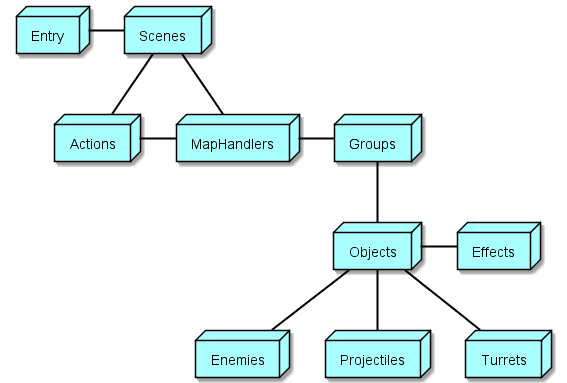
\includegraphics[width=1\textwidth]{kepek/uml/modules.png}
			\caption{Az alkalmazás moduljai és azok kapcsolati viszonya}
			\label{fig:uml:module}
		\end{figure}
		
		% uml képek pozíciója, ahol van overflow az jó-e?
		% kimaradt uml képek mellékletbe
		% \texttt{}-n belüli részeket nem engdei wrappelni, így kilógnak az oldalról
		
		\begin{MySubSection}{Entry modul}
			Az alkalmazás általános osztályai kaptak itt helyet.
			A modul osztálydiagramja a \myref{fig:uml:entry} ábrán látható.
			
			\begin{figure}[h!]
				\centering
				%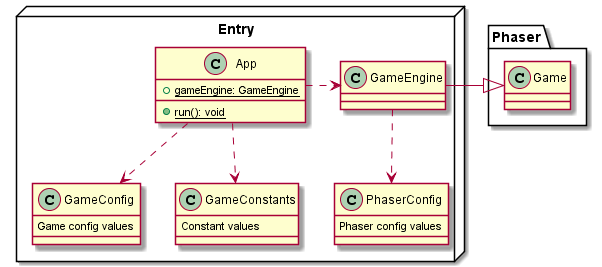
\includegraphics[scale=0.8]{kepek/uml/entry/entry.png}
				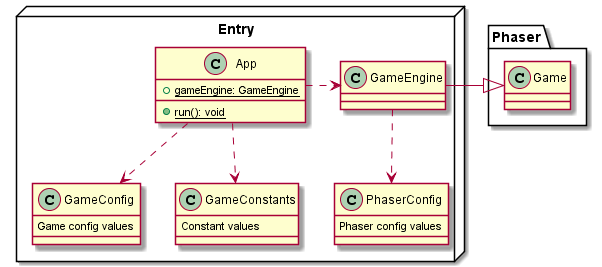
\includegraphics[width=1.05\textwidth]{kepek/uml/entry/entry.png}
				\caption{Az Entry modul osztálydiagramja}
				\label{fig:uml:entry}
			\end{figure}
		
			A modul osztályai az alábbi felsorolásban láthatóak:
			\begin{itemize}
				\item \texttt{App} - Az alkalmazás belépési pontját tartalmazó osztály, feladata a játékmotor (GameEngine) megfelelő paraméterekkel való inicializálása.
				
				\item \texttt{GameEngine} - A Phaser játékmotorának kibővítése, jelenleg nem tartalmaz semmilyen funkciót. A jövőbeli bővíthetőség végett került létrehozásra.
				
				\item \texttt{PhaserConfig} - A Phaserhez szükséges beállításokat tartalmazza, mint például: renderelő motor típusa, képernyő méretei, fizikai motor típusa és konfigurációja, valamint a megjelenítendő Scene-eket (képernyőket).
				
				\item \texttt{GameConfig} - A játékhoz használt konfigurálandó értékeket tartalmazza, mint például a pályaméretet, a tornyok sebzéseit, valamint árait.
				
				\item \texttt{GameConstants} - A játékhoz felhasznált konstans értékeket tárolja. Például a UI elemek z-index (mélység) értékeit, illetve a tilemap mezőinek értékeit.
			\end{itemize}
		\end{MySubSection}
	
		\begin{MySubSection}{Scenes modul}
			A különböző képernyőkkel kapcsolatos osztályok kaptak itt helyet.
			A modul osztálydiagramja a \myref{fig:uml:scene} ábrán látható.
			
			\begin{figure}[h!]
				\centering
				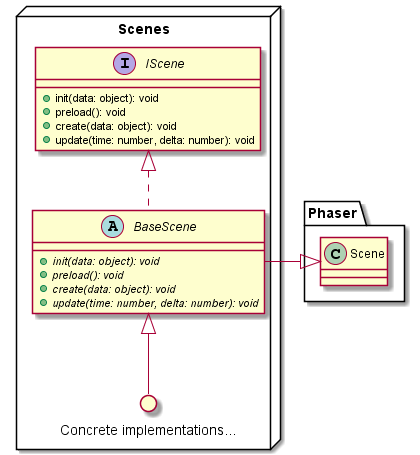
\includegraphics[scale=0.82]{kepek/uml/scenes/scene-pt1.png}
				\caption{A Scenes modul osztálydiagramja}
				\label{fig:uml:scene}
			\end{figure}
			
			A modul osztályai az alábbi felsorolásban láthatóak:
			\begin{itemize}
				\item \texttt{IScene} - Interface a Scene-ek által implementálandó metódusok megadására. A Phaser Scene implementációja megengedi ezen metódusok elhagyását, viszont az egységes kód érdekében inkább kötelezővé tettem őket.
				
				\item \texttt{BaseScene} - Absztrakt ősosztály melynek egyetlen feladata, hogy a konstruktorban megkapott azonosítót megfelelő formában továbbadja a Phasernek.
				
				\item \texttt{BootScene} - A legelső képernyő. Feladata a töltőképernyő hátterének betöltése, majd továbbnavigálás a \texttt{PreloadScene}-re.
				
				\item \texttt{PreloadScene} - A töltőképernyő osztálya. Feladata a szükséges fájlok, mint például képek, html oldalak betöltése, valamint a töltés állapotának kijelzése. A betöltés után átnavigál a \texttt{MainMenuScene}-re.
				
				\item \texttt{MainMenuScene} - A főmenü osztálya. Megjelenít egy beviteli mezőt, ahol a felhasználó megadhatja a pályageneráláshoz felhasználandó seed-et, egy gombot az előbbi érték randomizálásához, valamint még egy gombot a játék elindításához.
				
				\item \texttt{GameScene} - A legfontosabb képernyője a játéknak, ez tartalmazza magát a játékot. A játék logika nagy része viszont nem itt, hanem a \texttt{MapHandlers} modulba lett elhelyezve. Az osztály feladatai az előbb említett modul segítségével a pálya generálása és megjelenítése, valamint a felhasználói felület létrehozása és kezelése. Vagyis csak a kifejezetten a megjelenítéshez köthető részek kerültek ide, például a belső logika már nem.
				
				\item \texttt{GameOverScene} - A játék vége után ez a képernyő jeleníti meg a játékos által elért pontszámot, illetve egy gombbal lehetőséget is ad visszatérni a főmenübe.
			\end{itemize}
			
			Az UML ábráról lemaradt osztályok megtalálhatóak a mellékletek között.
			% extra képek scene-2 -> scene-6
		\end{MySubSection}
	
		\begin{MySubSection}{Actions modul}
			A felhasználói interakcióval kapcsolatos események osztályai kaptak itt helyet.
			A modul osztálydiagramja a \myref{fig:uml:action} ábrán látható.
			
			\begin{figure}[h!]
				\centering
				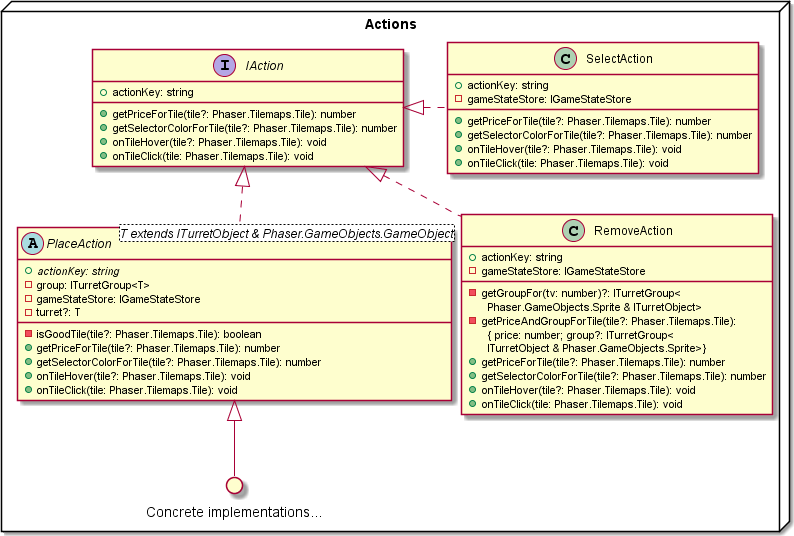
\includegraphics[width=1.12\textwidth]{kepek/uml/actions/action-pt1.png}
				\caption{Az Actions modul osztálydiagramja}
				\label{fig:uml:action}
			\end{figure}
			
			A modul osztályai az alábbi felsorolásban láthatóak:
			\begin{itemize}
				\item \texttt{IAction} - Interface ami a UI-nál és a pályakezelésnél szükséges metódusokat tartalmazza. Ezek a metódusok határozzák meg a megjelenítendő árat (getPriceForTile), a kijelölés színét (getSelectorColorForTile), hogy mi történjen ha kattintunk az egérrel (onTileClick), és azt, hogy mi történjen ha új helyre mozgatjuk az egeret (onTileHover).
				
				\item \texttt{SelectAction} - A pálya mezőinek kijelölését valósítja meg. Különböző színekkel jelzi, ha egy mező kijelölhető vagy sem, illetve plusz információt mutat a mezőről ha ki van jelölve.
				
				\item \texttt{RemoveAction} - A feladata a pályán lévő objektumok eltávolítása. Az előzőhöz hasonlóan különböző színnel jelzi, ha a mezőn van eltávolítható objektum, vagy sem. Jelzi továbbá a művelet költségét, kattintás esetén eltávolítja az objektumot a mezőről, illetve jóváírja az összeget a játékosnak.
				
				\item \texttt{PlaceAction} - Absztrakt osztály, a tornyok lerakását szolgálja. A többihez hasonló módon jelzi az aktuális árat és a lerakhatóságot. Kattintásra elhelyezi a tornyot, illetve levonja az összeget a játékostól. A torony konkrét típusát a leszármazottak határozzák majd meg.
				
				\item \texttt{Place<T>Action} - Ezek az osztályok a \texttt{PlaceAction}-t bővítik ki. Egyetlen feladatuk a lerakandó torony típusának meghatározása. Példa: PlaceTurretBulletMk1Action.
			\end{itemize}
			
			Az UML ábráról lemaradt osztályok megtalálhatóak a mellékletek között.
			% extra képek action-2 -> action-6
		\end{MySubSection}
	
		\begin{MySubSection}{MapHandlers modul}
			A pályával és annak kezelésével kapcsolatos osztályok kaptak itt helyet.
			A modul osztálydiagramja a \myref{fig:uml:map} ábrán látható.
			
			A modul osztályai az alábbi felsorolásban láthatóak:
			\begin{itemize}
				\item \texttt{IMapGenerator} - Interface, ami a pálya generálásához szükséges metódust definiálja. A többi osztályban nem a konkrét implementáció, hanem ez az interface van használva.
				
				\item \texttt{MapGenerator} - A pálya generálását megoldó osztály. Fontos, hogy adott kezdőértékhez (úgynevezett ``seed''-hez) ugyanazt a pályát generálja mindig. A pályagenerálás során egy útvonalat is generál, amin az ellenségek fognak majd haladni. A pálya mezőinek lehetséges értékei előre meghatározottak, melyek a \texttt{GameConstants} osztályban lettek definiálva.
				
				\item \texttt{IEnemySpawner} - Interface, ami az ellenségek létrehozásához, és a játék köreinek kezeléséhez szükséges metódusokat definiálja. Ezeket, az \texttt{update} metódus kivételével, főként a UI használja.
				
				\item \texttt{EnemySpawner} - Elsődlegesen az ellenségek létrehozásáért felel, de feladata még a körök kezelése, az ellenségek számának és erejének fokozatos növelése is. Működése közvetlenül a \texttt{GameStateStore}-al van összefüggésben.
				
				\item \texttt{IGameStateStore} - Talán a legtöbbet használt interface az alkalmazásban. Számos metódust definiál a UI és a többi modul felé.
				
				\item \texttt{GameStateStore} - Ebbe az osztályba került a logika nagy része. Ez kezeli az objektum-csoportokat, az életerőt, a pénzt, a pontszámot, a pályát és az útvonalat. A \texttt{EnemySpawner}-en keresztül az ellenségeket és a köröket is ez kezeli. Számos úgynevezett ``callback'' metódust is tartalmaz melyek segítségével a UI frissíteni tudja a megjelenített adatokat.
			\end{itemize}
		
			\begin{figure}[H]
				\centering
				%includegraphics[width=1.1\textwidth]{kepek/uml/maphandlers/map.png}
				\makebox[1.05\textwidth][c]{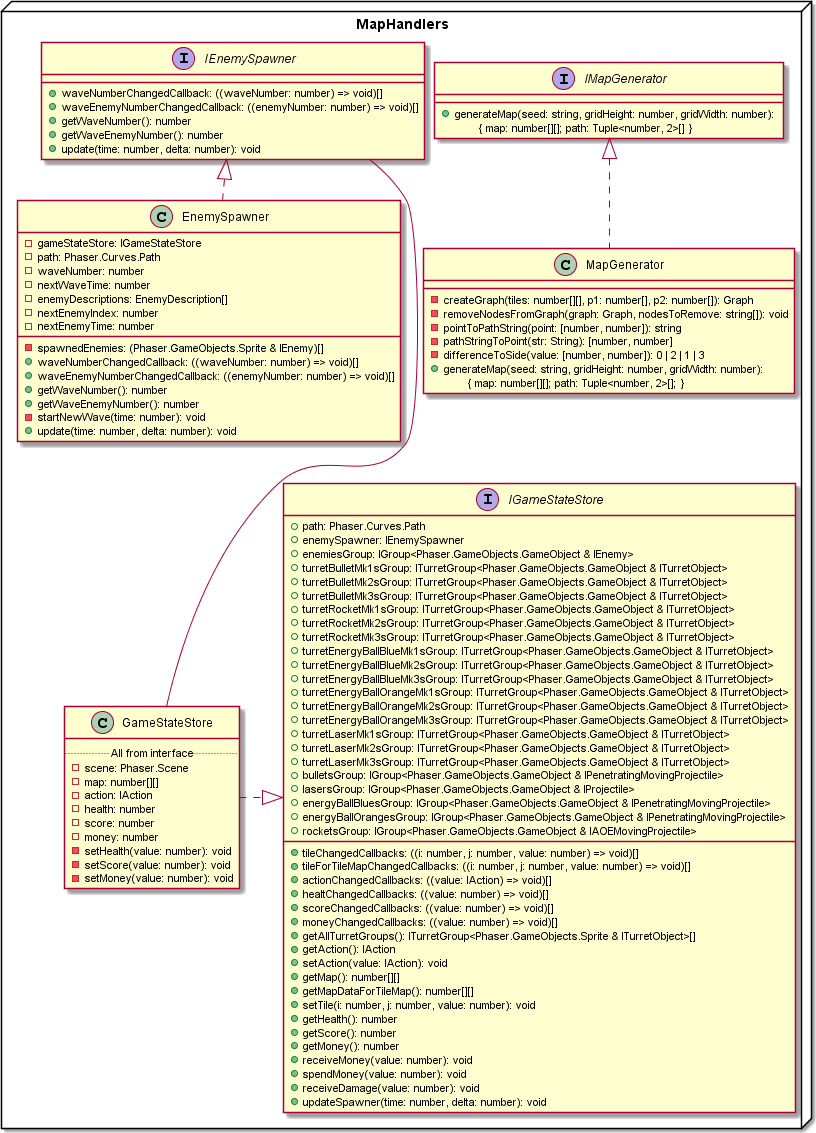
\includegraphics[width=1.1\textwidth]{kepek/uml/maphandlers/map.png}}
				\caption{A MapHandlers modul osztálydiagramja}
				\label{fig:uml:map}
			\end{figure}
		\end{MySubSection}
	
		\begin{MySubSection}{Groups modul}
			Az objektum-csoportokkal kapcsolatos osztályok kaptak itt helyet.
			A modul osztálydiagramja a \myref{fig:uml:group} ábrán látható.
	
			\begin{figure}[h!]
				\centering
				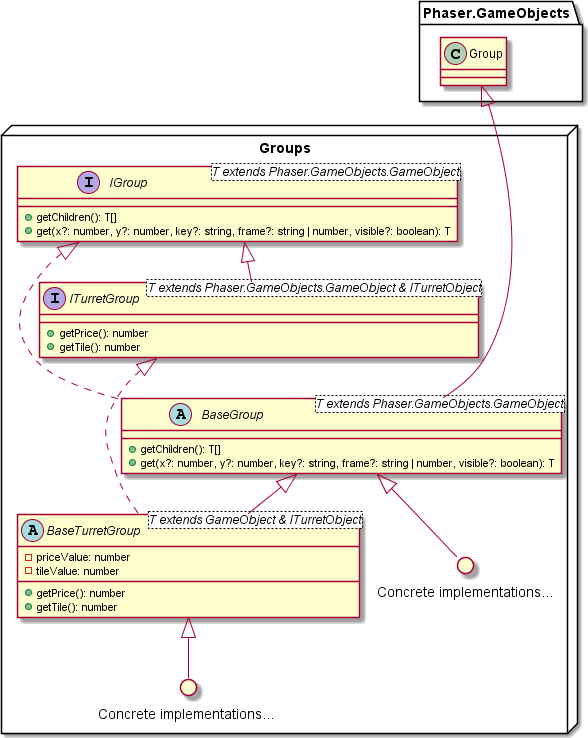
\includegraphics[width=1\textwidth]{kepek/uml/groups/group-pt1.png}
				\caption{A Groups modul osztálydiagramja}
				\label{fig:uml:group}
			\end{figure}
			
			A modul osztályai az alábbi felsorolásban láthatóak:
			\begin{itemize}
				\item \texttt{IGroup} - Interface ami az objektum-csoportok által nyújtott legszükségesebb metódusokat tartalmazza. Gyakorlatilag a Phaser által definiált metódusokat írja felül, mivel azok nem megfelelő típussal rendelkeznek (nem generikusak).
				
				\item \texttt{BaseGroup} - Az \texttt{IGroup} interface implementációja, az ott említett dolgokat valósítja meg. A Phaser \texttt{Group} osztályának a kibővítése.
				
				\item \texttt{ITurretGroup} - Az \texttt{IGroup} interface kibővítése a tornyoknál egyedileg szükséges dolgokkal, melyek a torony ára és a mező értéke.
				
				\item \texttt{BaseTurretGroup} - Absztrakt osztály, mely az \texttt{ITurretGroup} interface-t valósítja meg. A konkrét árat és mező értéket a leszármazottak fogják meghatározni.
				
				\item \texttt{<T>Group} - A lövedékek és az ellenségek konkrét csoportjai. Az ősosztály felé a kezelendő objektum osztályát határozzák meg. Példa: \texttt{BulletGroup}
				
				\item \texttt{Turret<T>Group} - A tornyok konkrét csoportjai. Az ősosztály felé a kezelendő torony osztályát, árát és mezőértékét határozzák meg. Példa: \texttt{Turret\-Bullet\-Mk1\-Group}
			\end{itemize}
			
			Az UML ábráról lemaradt osztályok megtalálhatóak a mellékletek között.
			% extra képek group-2 -> group-7
		\end{MySubSection}
	
		\begin{MySubSection}{Objects modul}
			Az objektumokkal kapcsolatos osztályok egy része kapott itt helyet.
			A modul osztálydiagramja a \myref{fig:uml:object} ábrán látható.
			
			\begin{figure}[H]
				\centering
				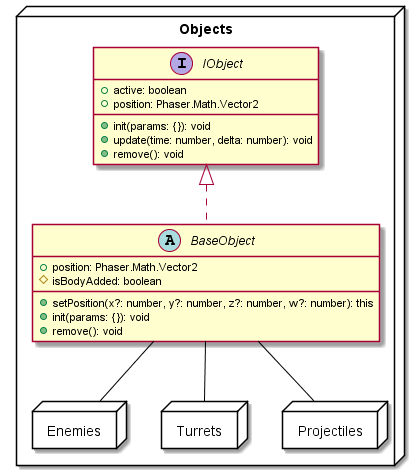
\includegraphics[width=0.72\textwidth]{kepek/uml/objects/object.png}
				\caption{Az Objects modul osztálydiagramja}
				\label{fig:uml:object}
			\end{figure}
			
			A modul osztályai az alábbi felsorolásban láthatóak:
			\begin{itemize}
				\item \texttt{IObject} - Interface ami az objektumok életciklus metódusait (init, update, remove), és alapvetően tagjait (position, active) határozza meg.
				
				\item \texttt{BaseObject} - Absztrakt osztály ami az előző interface tagjainak inicializálását, frissítését, és resetelését végzi el oly módon, hogy az tovább bővíthető legyen a későbbiekben. Ez a bővítés az \texttt{Enemies}, a \texttt{Projectiles} és a \texttt{Turrets} modulokban történik meg.
				
			\end{itemize}
		\end{MySubSection}
	
		\begin{MySubSection}{Effects modul}
			Az effektekkel kapcsolatos osztályok kaptak itt helyet.
			A modul osztálydiagramja a \myref{fig:uml:effect} ábrán látható.
			
			\begin{figure}[h!]
				\centering
				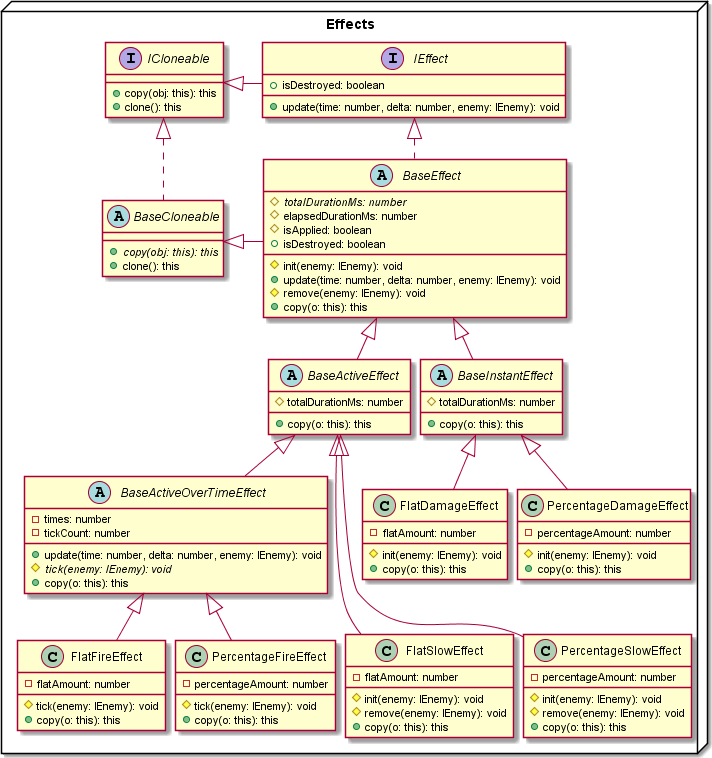
\includegraphics[width=1.1\textwidth]{kepek/uml/effects/effect.png}
				\caption{Az Effects modul osztálydiagramja}
				\label{fig:uml:effect}
			\end{figure}
			
			A modul osztályai az alábbi felsorolásban láthatóak:
			\begin{itemize}
				\item \texttt{IEffect} - Az effektek használatához szükséges tagokat és metódusokat definiálja, melyek az update és az isDestroyed. Ezeket a tornyok, a lövedékek és az ellenségek fogják használni.
				
				\item \texttt{ICloneable} - A klónozáshoz szükséges metódusokat definiáló interface. Alapvetően azért van a klónozásra szükség, mert a tornyoknak valahogy át kell adniuk a lövedékek számára az effekteket, anélkül, hogy az eredeti változat módosulhasson.

				\item \texttt{BaseCloneable} - Az előző interface-t félig megvalósító osztály. Implementálja a clone metódust a copy metódus használatával melyet a leszármazottaknak kell majd implementálni.

				\item \texttt{BaseEffect} - Absztrakt osztály, mely az effektek ellenségre való alkalmazását, levételét, és frissítését valósítja meg oly módon, hogy az a leszármazottak által bővíthető legyen.

				\item \texttt{BaseInstantEffect} - Absztrakt osztály, amely olyan effektet valósít meg, ami azonnali hatású, vagyis amint felkerül az ellenségre azonnal el is kerül róla.

				\item \texttt{FlatDamageEffect} - A \texttt{BaseInstantEffect} egyik leszármazott osztálya. Azonnali hatású, fix értékű sebzést alkalmaz az ellenségre.

				\item \texttt{PercentageDamageEffect} - A \texttt{BaseInstantEffect} egyik leszármazott osztálya. Azonnali hatású, százalékos értékű sebzést alkalmaz az ellenségre. A sebzés mindig az ellenség aktuális éltereje alapján történik.

				\item \texttt{BaseActiveEffect} - Absztrakt osztály, amely olyan effektet valósít meg, ami fix ideig érvényes.

				\item \texttt{FlatSlowEffect} - A \texttt{BaseActiveEffect} egyik leszármazott osztálya. Pár másodpercig tartó fix értékű lassítást alkalmaz az ellenségre.

				\item \texttt{PerncetageSlowEffect} - A \texttt{BaseActiveEffect} egyik leszármazott osztálya. Pár másodpercig tartó százalékos értékű lassítást alkalmaz az ellenségre. A lassítás mindig az ellenség aktuális sebessége alapján történik. (A játékban végül nem használt.)

				\item \texttt{BaseActiveOverTimeEffect} - Absztrakt osztály, amely olyan effektet valósít meg, ami fix ideig érvényes, emellett adott időközönként alkalmaz az ellenségre hatásokat.

				\item \texttt{FlatFireEffect} - A \texttt{BaseActiveOverTimeEffect} egyik leszármazott osztálya. A tűzsebzést hivatott modellezni. Pár másodpercig tartó fix értékű sebzést alkalmaz az ellenségre minden időközben.
				
				\item \texttt{PercentageFireEffect} - A \texttt{BaseActiveOverTimeEffect} egyik leszármazott osztálya. A tűzsebzést hivatott modellezni. Pár másodpercig tartó százalékos értékű sebzést alkalmaz az ellenségre minden időközben. A sebzés mindig az ellenség aktuális éltereje alapján történik. (A játékban nem használt.)
			\end{itemize}
		\end{MySubSection}
	
		\begin{MySubSection}{Projectiles modul}
			A lövedékekkel kapcsolatos osztályok kaptak itt helyet.
			A modul osztálydiagramja a \myref{fig:uml:projectile} ábrán látható.
		
			\begin{figure}[h!]
				\centering
				%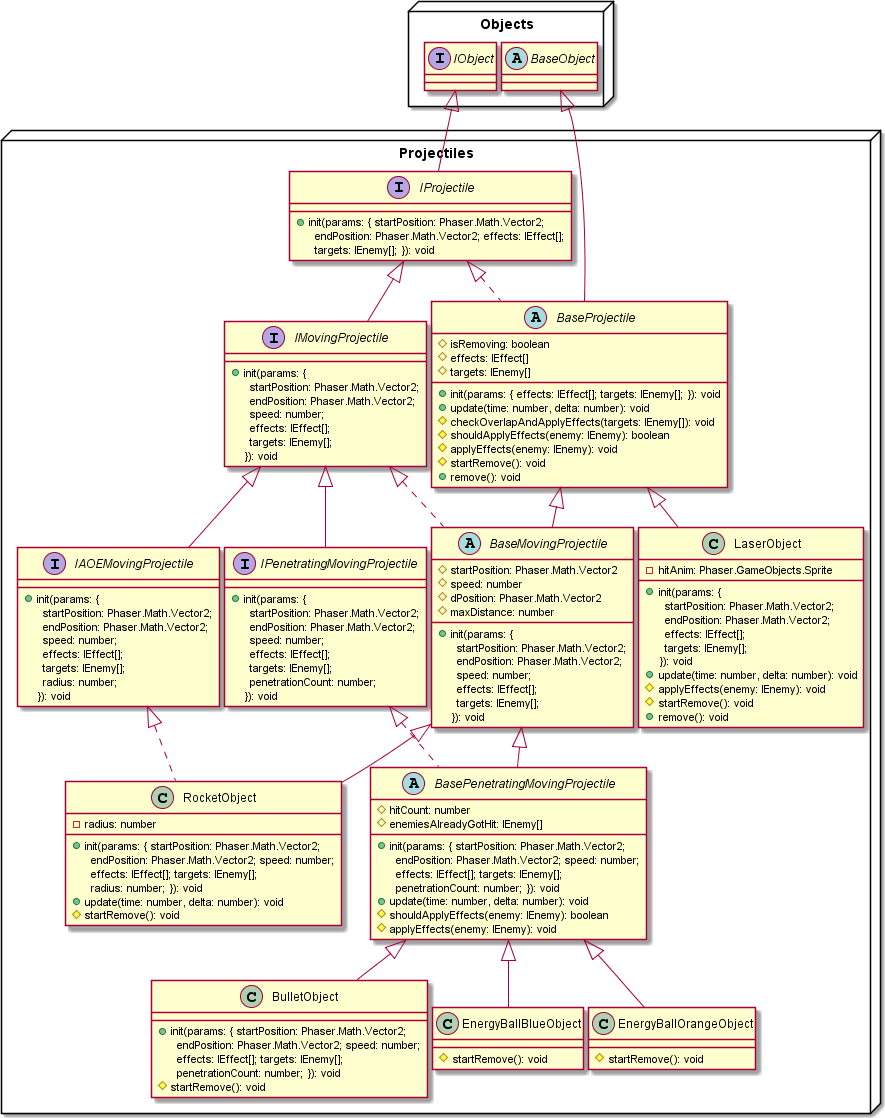
\includegraphics[width=1.1\textwidth]{kepek/uml/projectiles/projectile.png}
				\makebox[1.1\textwidth][c]{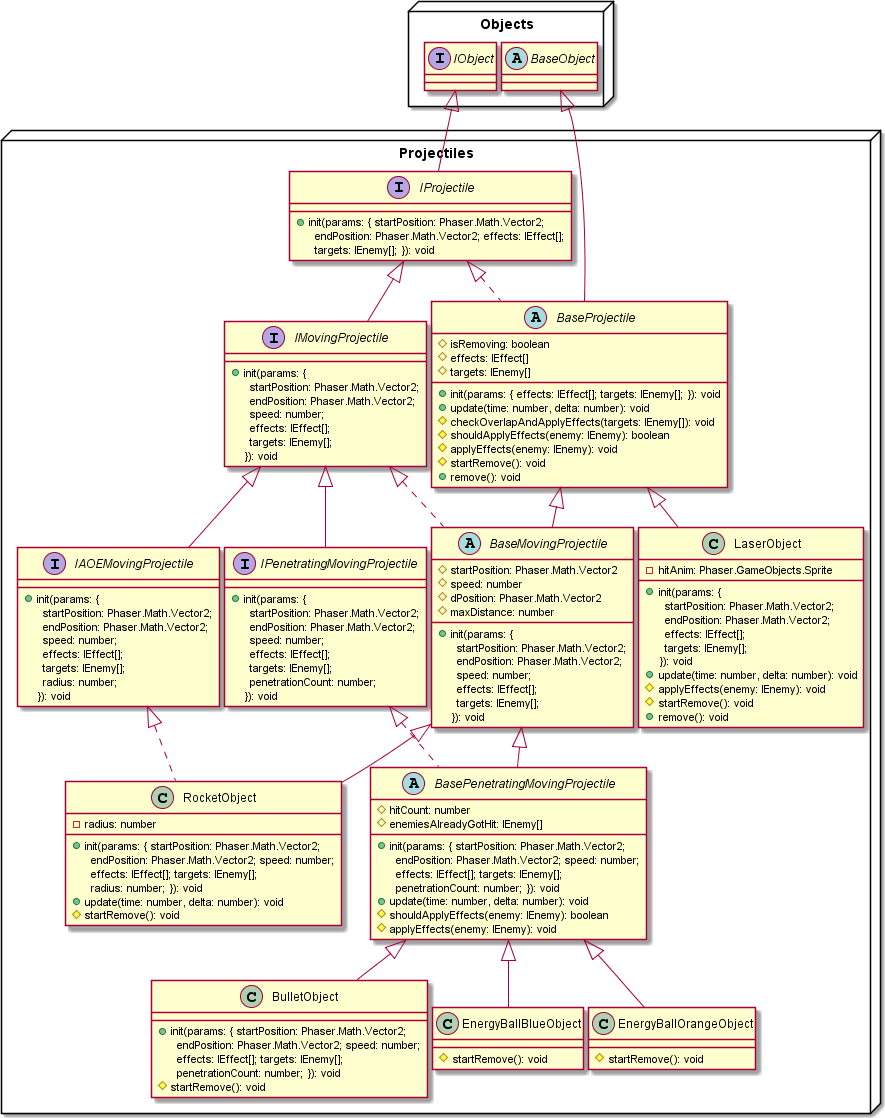
\includegraphics[width=1.175\textwidth]{kepek/uml/projectiles/projectile.png}}
				\caption{A Projectiles modul osztálydiagramja}
				\label{fig:uml:projectile}
			\end{figure}
			
			A modul osztályai az alábbi felsorolásban láthatóak:
			\begin{itemize}
				\item \texttt{IProjectile} - Interface, ami a lövedékek általános inicializáló paramétereit határozza meg. Kibővíti az \texttt{IObject} interface-t.

				\item \texttt{BaseProjectile} - Absztrakt osztály, ami az \texttt{IProjectile}-nak megfelelően implementálja a lövedékek általános funkcióit és tulajdonságait oly módon, hogy az később bővíthető legyen.

				\item \texttt{LaserObject} - Lézersugarat reprezentáló osztály. Ez egy nem mozgó és azonnal sebző lövedék típus, mely pontosan egy konkrét ellenfelet sebezhet csak. Megjelenítéshez animációt is tartalmaz. A \texttt{BaseProjectile}-ból származik le.

				\item \texttt{IMovingProjectile} - Interface, ami a mozgó lövedékek plusz inicializáló paramétereivel bővíti ki az \texttt{IProjectile} interface-t.

				\item \texttt{BaseMovingProjectile} - Absztrakt osztály, ami a \texttt{BaseProjectile}-t bővíti ki a mozgó lövedékek tulajdonságainak megfelelően. Ez az osztály is a későbbi bővíthetőséget figyelembe véve készült.

				\item \texttt{IAOEMovingProjectile} - Interface, ami a területi sebzést okozó lövedékeknél használatos paraméterekkel bővíti ki a \texttt{IMovingProjectile}-t.

				\item \texttt{RocketObject} - A rakétát megtestesítő osztály. A \texttt{BaseMovingProjectile}-ból származik le. Feladata a rakétákra jellemző területi sebzés megvalósítása, és animáció kezelése.

				\item \texttt{IPenetratingMovingProjectile} - Interface, ami kibővíti a \texttt{IMovingProjectile} interface-t, az átütőképességgel rendelkező lövedékekhez szükséges paraméterekkel.

				\item \texttt{BasePenetratingMovingProjectile} - Absztrakt osztály, ami a \texttt{Base\-Moving\-Projectile}-ból származik le. Feladata az átütőképességgel rendelkező lövedékek számára egy közös ős biztosítása. Kezeli a lövedék élettartamát, illetve metódusokat szolgáltat az eltalált ellenségek nyomonkövetésére.

				\item \texttt{BulletObject} - Az egyszerű lövedéket megvalósító osztály. A \texttt{Base\-Penetrating\-Moving\-Projectile}-ból származik le. Feladatai az egyedi animáció és megjelenés biztosítása.

				\item \texttt{EnergyBallBlueObject} - A kék színű energia-lövedéket megvalósító osztály. A \texttt{Base\-Penetrating\-Moving\-Projectile}-ból származik le. Feladatai az egyedi animáció és megjelenés biztosítása.

				\item \texttt{EnergyBallOrangeObject} - A sárga színű energia-lövedéket megvalósító osztály. A \texttt{Base\-Penetrating\-Moving\-Projectile}-ból származik le. Feladatai az egyedi animáció és megjelenés biztosítása.
							
			\end{itemize}
		\end{MySubSection}

		\begin{MySubSection}{Turrets modul}
			A tornyokkal kapcsolatos osztályok kaptak itt helyet.
			A modul osztálydiagramja a \myref{fig:uml:turret} ábrán látható.
			
			\begin{figure}[h!]
				\centering
				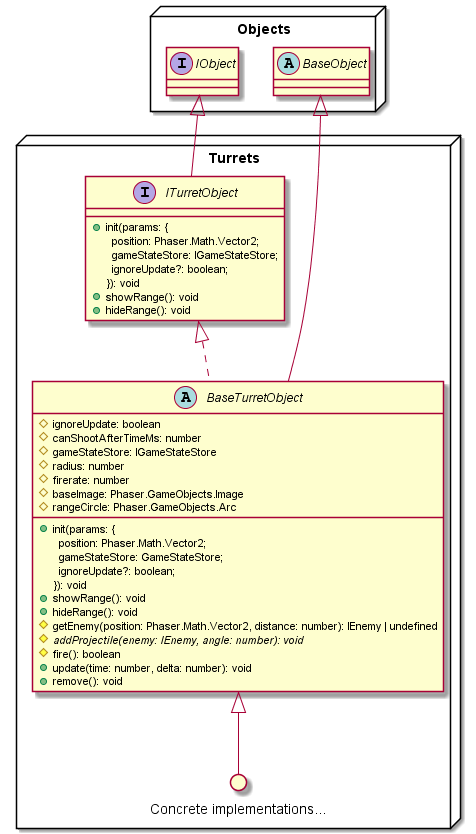
\includegraphics[width=0.656\textwidth]{kepek/uml/turrets/turret-pt1.png}
				\caption{A Turrets modul osztálydiagramja}
				\label{fig:uml:turret}
			\end{figure}
			
			A modul osztályai az alábbi felsorolásban láthatóak:
			\begin{itemize}
				\item \texttt{ITurretObject} - Interface, ami a tornyok használatához szükséges metódusokat definiálja, mint például a hatótáv indikátor megjelenítése és elrejtése. Az \texttt{IObject} interface-t bővíti ki.
				
				\item \texttt{BaseTurretObject} - Absztrakt osztály, ami a tornyok logikájának nagyrészét tartalmazza. Kezeli a torony létrehozását, eltávolítását, az ellenségek kiválasztását, illetve megtámadását, valamint a hatótáv jelölő megjelenítését és eltávolítását. A konkrét lövedék típusokat az alosztályok fogják meghatározni.
				
				\item \texttt{Turret<T>Object} - A konkrét torony típusokat megvalósító osztályok. Közös ősük a \texttt{BaseTurretObject}-t. Feladatuk a torony tulajdonságainak (hatótáv, tűzgyorsaság), a megjelenítésének és a konkrét lövedék típusainak a meghatározása.
				
			\end{itemize}
			
			Az UML ábráról lemaradt osztályok megtalálhatóak a mellékletek között.
			% extra képek turret-2 -> turret-6
		\end{MySubSection}

		\begin{MySubSection}{Enemies modul}
			Az ellenségekkel kapcsolatos osztályok kaptak itt helyet.
			A modul osztálydiagramja a \myref{fig:uml:enemy} ábrán látható.
				
			\begin{figure}[h!]
				\centering
				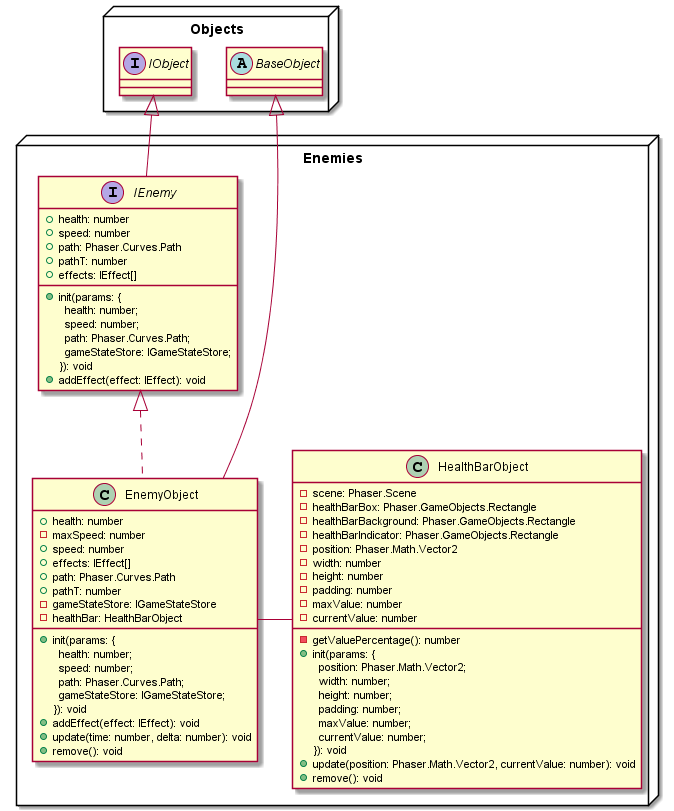
\includegraphics[width=0.906\textwidth]{kepek/uml/enemies/enemy.png}
				\caption{Az Enemies modul osztálydiagramja}
				\label{fig:uml:enemy}
			\end{figure}
			
			A modul osztályai az alábbi felsorolásban láthatóak:
			\begin{itemize}			
				\item \texttt{IEnemy} - Interface, a többi osztály számára fontos metódusokat és tulajdonságokat definiálja az ellenségekhez. Kapcsolatban van az \texttt{Effects} modullal is.
				
				\item \texttt{EnemyObject} - Esetünkben az egyetlen konkrét ellenfelet reprezentáló osztály. Feladatai az ellenség életének és egyéb tulajdonságainak a számontartása, az effektek kezelése, a megjelenítés és animációk meghatározása, illetve az ellenség mozgatása az útvonalon. Szoros kapcsolatban áll a \texttt{HealthBarObject} osztállyal.
				
				\item \texttt{HealthBarObject} - Az ellenségek életerejét megjelenítő osztály. Létrehozása után követnie szükséges az adott ellenfelet, mely az egyik feladata. Feladata még az életerő megfelelő megjelenítése, melyet kívülről testreszabható módon végez.
				
			\end{itemize}
		\end{MySubSection}
	
	\end{MySection}
	
	\begin{MySection}{Megvalósítás}	
		Ebben a fejezetben a játék fejlesztéséről, a közben felmerült problémákról, illetve az érdekesebb kódrészletek bemutatásáról lesz szó.
		
		\begin{MySubSection}{A program struktúrája}
			Mint említettem, az alkalmazást a Webpack segítségével készítettem el. Az ezáltal használt forrásfájlok az \texttt{src} mappában kerültek elhelyezésre. Ezek között a forrásfájlok között találhatóak statikus és script fájlok is, melyek a típusuknak megfelelően további almappákba lettek csoportosítva.
			Ezek a következőek:
			
			\begin{itemize}
				\item \texttt{html} - A HTML fájlok kerültek ide. Itt található az \texttt{index.html} is, ami az alkalmazás kiinduló pontja, ezt tölti be legelőször a böngésző és itt kerül belinkelésre magának a játéknak a kódja is. Az itt található többi fájl a Phaser által kerül megjelenítésre a játékon belül.
				
				\item \texttt{css} - A CSS (Cascading Style Sheet) fájlok kerültek ide, ezek tartalmazzák a HTML fájlokhoz esetlegesen szükséges stílusdefiníciókat.
				
				\item \texttt{fonts} - Az egyedi betűkészlet fájloknak lenne a helye, de jelenleg nem használok ilyeneket, ezért ez a mappa üres.
				
				\item \texttt{images} - Az alkalmazásban használt képek helye. Ide kerültek mind a HTML-ben, mind a Phaser által használt képek és sprite sheetek. A sprite sheetekhez szükséges JSON fájlok is ide kerültek, mivel azok szorosan hozzájuk köthetőek.
				
				\item \texttt{scripts} - Itt találhatóak a tényleges kódot tartalmazó fájlok, vagyis a JavaScript és TypeScript állományok, melyek további almappákban lettek elhelyezve. Az almappák a következőek:
				\begin{itemize}
					\item \texttt{\_\_doc\_\_} - Az dokumentációs fájlok, vagyis a generált UML diagramok és forrásfájljaiknak a helye. Ezeket a \texttt{tplant} NPM-es csomag és a \url{www.plantuml.com} segítségével készítettem el.
					
					\item \texttt{\_\_test\_\_} - A tesztállományok helye.
					
					\item \texttt{api} - Az alkalmazásban felhasznált interface-ek, illetve TypeScript típusok helye.
					
					\item \texttt{impl} - A tényleges implementáció helye. Tartalma az absztrakt és a konkrét osztályok.
				\end{itemize}
			\end{itemize}
		\end{MySubSection}
		
		\begin{MySubSection}{Az assetek}
			Az assetek alatt a játékoknál minden olyan fájlt értünk, ami bekerül a termékbe, de nem kifejezetten forrásfájl. Ilyenek például a képek, animációk, hangeffektek, térképek, satöbbi. \cite{game_development_terms} Esetemben ezek meglepően nagy fejtörést jelentettek, több időt kellett rájuk szánnom, mint reméltem. Ennek oka, hogy sok idő volt megfelelő képeket, animációkat találni a játékhoz, mivel kevés ingyenes és egyben jól használható található az interneten. Legtöbbjük vagy nem ingyenes, vagy hiányzik belőlük néhány rész (pl.: lövedékhez animáció), vagy egyszerűen nem kompatibilis másokkal. Éppen ezért végül amellett döntöttem, hogy több forrásból összeillesztve készítem el az alkalmazást. Ehhez természetesen elkerülhetetlen volt, hogy módosításokat kelljen végeznem a fájlokon, illetve néhány esetben még bizonyos részeket nekem kellett létrehoznom is (a rakétavető lövedékét). Az így elvégzett módosítások a következőek voltak: egységesíteni kellett a képek méreteit, formátumát, a sprite sheetek elrendezését, kombinálni különböző részeket, a képen belül megfelelően pozícionálni az objektumokat, illetve közel egységessé tenni a különböző elemek színvilágát, stílusát. Ezekben nagy segítségemre voltak a \myref{Felhasznált eszközök, technológiák} fejezetben már említett ``\texttt{Photopea}'', ``\texttt{Free Sprite Sheet Packer}'' és a ``\texttt{Sprite sheet cutter}'' alkalmazások.
			% cite https://unity.com/how-to/beginner/game-development-terms
		\end{MySubSection}
		
		\begin{MySubSection}{A Phaser fizikai motorjai}
			A Phaser-ben két különböző fizikai motorból lehet választani, név szerint az \textit{Arcade} és a \textit{Matter} közül. A Phaser ajánlása szerint az \textit{Arcade} motort érdemes használni mindaddig, amíg valami miatt nincs szükségünk a másikra, mivel az állítólag sokkal gyorsabb és egyszerűbb kezelni. Ennek megfelelően én is az \textit{Arcade} motort használtam és tényleg egyszerűnek tűnt a kezelése mindaddig, amíg nem futottam bele egy komoly hiányosságba. Lényegében arról volt szó, hogy az \textit{Arcade} motor azért gyorsabb (és egyszerűbb) mint a másik, mivel ez csak az úgynevezett AABB (koordináta tengelyekkel párhuzamos) befoglaló testekkel tud számolni. Ebből kifolyólag kiderült számomra, hogy a lövedékek kezelése ily módon nem fog működni, mivel ez azt jelentené, hogy nem lehetne elforgatni semmit, tehát a lövedékek nem mehetnének átlósan, vagy más koordináta tengelyekkel nem párhuzamos irányba. Ez elég sajnálatos volt, mivel ekkorra már a játék nagyrésze elkészült, és ezeket a részeket mind át kellett írni az új motor használatának megfelelően.
			
			További probléma volt, hogy a Phaser egyik frissen kiadott verziójába belekerült egy olyan hiba a \textit{Matter} motorral kapcsolatban, ami problémássá tette a használatát a csoportokkal (group-okkal). Itt arról volt szó, hogy optimalizáció gyanánt a fizikai motor számon tartotta az előző ütközéseket az adott objektumok között, és ezeket az előzményeket használta mindaddig, amíg bizonyos feltételek miatt mindenképp újra nem kellett számolni az értékeket. A probléma a csoportokban kezelt objektumoknál jelentkezett, mivel ezek az objektumok nem törlődnek ténylegesen, csak inaktív állapotba kerülnek egy esetleges eltávolítás esetén, és ebben az inaktív állapotban nem törlődnek az előzményeik, így amikor újra aktiválva lett az adott objektum, immár új pozícióval és értékekkel, akkor az ütközésvizsgálat esetén a motor felhasználta ezeket az előzményeket, mely így könnyedén futásidejű hibát eredményezett a teljes alkalmazás összeomlásával egyetemben. Szerencsére miután fényt derítettem a hiba okára, megoldást is találtam rá: az aktiválás során a fizikai motor által használt testet újra létrehozom ezáltal törölve annak előzményeit. Remélhetőleg egy jövőbeni kiadásában a Phaser-nek ezt javítani fogják, de addig is ezzel az javítással megkerülhető a probléma.
		\end{MySubSection}
		
		\begin{MySubSection}{A pályagenerálás}
			A pályagenerálás egy viszonylag bonyolult része a programnak, éppen ezért ehhez készítettem külön teszteket is a helyes működés biztosítása érdekében.
			A koncepció az volt, hogy megadott seed (kezdő random érték) használatával fix méretű pályát és útvonalat tudjak generálni. A pályagenerálás része egyszerű volt. Egy seed-elhető random generáló package-et használva minden mezőhöz egy véletlenszerű értéket párosítottam $0$ és $1$ között. Ezt követően, ahogy az az alábbi kódrészletben is látható, átkonvertáltam ezeket az értékeket a konkrét mezőértékekre.
			\begin{javascript}
for (let i = 0; i < gridWidth; i++) {
	for (let j = 0; j < gridHeight; j++) {
		if (tiles[i][j] < 0.7) {
			tiles[i][j] = §\color{jsConst}TILE\_EMPTY§ + §\color{jsConst}ROTATION\_ZERO§;
		} else if (tiles[i][j] < 0.85) {
			tiles[i][j] = §\color{jsConst}TILE\_CRATERS§ + §\color{jsConst}ROTATION\_ZERO§;
		} else {
			tiles[i][j] = §\color{jsConst}TILE\_TREES§ + §\color{jsConst}ROTATION\_ZERO§;
		}
	}
}
			\end{javascript}
			Esetünkben a $0.7$- nél kisebb értékek az üres mezők lesznek, a $0.7$ és $0.85$ közé esők a kráterek, a maradékok pedig erdők.
			
			A nehezebb rész az útvonal generálása volt, hiszen a gyakorlati hasznosításhoz több dolognak is meg kell felelnie az útvonalnak. Néhány ilyen kritérium a következő:
			\begin{itemize}
				\item Legyen változatos az útvonal.
				\item Ne legyenek kereszteződések.
				\item Lehetőség szerint legyen elegendő hely az útvonal mentén tornyok lerakására.
			\end{itemize}
			A megvalósítás során az alábbi ötletet használtam fel: a kigenerált pálya értékeit (még a konvertálás előtt) fel lehetne használni súlyokként valamilyen útkereső algoritmushoz. Így is tettem és a Dijkstra algoritmust \cite{dijkstra} felhasználva kerestem a legrövidebb utat a pálya bal felső sarkából a bal alsóba. Egy adott él súlyát a két mezőérték különbsége határozta meg. Az algoritmust nem én implementáltam, helyette egy külső csomagot használtam mely ``node-dijkstra'' néven fut. Itt bele is futottam az első hibába, hiszen az algoritmus nem enged meg negatív súlyokat, ami esetünkben könnyedén előállhat, hiszen a véletlenül generált mezőértékeknek $0$ és $1$ közé kell esniük, így attól függően, hogy melyiket melyikből vonjuk ki legrosszabb esetben $+1$ és $-1$ lesz a végeredmény. Ezt egy túlzó $+5$-ös eltolással orvosoltam, amitől már $+4$ és $+6$ közé esett mindegyik súlyérték. Így már sikerült útvonalat generálni, de azt tapasztaltam, hogy dacára a véletlen értékeknek mégis túlságosan egysíkú az eredmény. Így hát úgy döntöttem ezt elkerülendő hozzáadok még fixen érintendő pontokat az útvonalhoz, egyet a jobb felső negyedbe, egyet pedig a bal alsó negyedbe. 
			\begin{javascript}
let path: §\color{jsType}string§[] = [];
for (let i = 0; i < §\color{jsConst}fixPoints§.length - 1; i++) {
	const §\color{jsConst}startPoint§ = §\color{jsConst}fixPoints§[i];
	const §\color{jsConst}endPoint§ = §\color{jsConst}fixPoints§[i + 1];
	
	const §\color{jsConst}graph§ = this.§\color{jsMethod}createGraph§(tiles, §\color{jsConst}startPoint§, §\color{jsConst}endPoint§)
	this.§\color{jsMethod}removeNodesFromGraph§(§\color{jsConst}graph§, path);
	const §\color{jsConst}partialPath§: §\color{jsType}string§[] = §\color{jsConst}graph§.§\color{jsMethod}path§(
		this.§\color{jsMethod}pointToPathString§(§\color{jsConst}startPoint§),
		this.§\color{jsMethod}pointToPathString§(§\color{jsConst}endPoint§),
	);
	
	path.§\color{jsMethod}push§(...§\color{jsConst}partialPath§);
}

//removes duplicated inner fixpoints
path = path.§\color{jsMethod}filter§(
	(item, index, array) => array.§\color{jsMethod}indexOf§(item) === index
);
			\end{javascript}
			A kódrészletben látható, ahogy a fix pontokon végighaladva páronként megkeresem a köztük lévő legrövidebb utat. Az is látható, hogy a már érintett pontokat eltávolítom a keresési gráfból, ezáltal megakadályozva a kereszteződések létrejöttét. Felmerült egy olyan probléma is, hogy ha az aktuális útszakasz pont a pálya szélén megy végig, akkor elképzelhető, hogy nem létezik útvonal a következő fix ponthoz. Ezt elkerülendő a közbenső 2 pont generálásakor a pálya szélét nem veszem figyelembe, illetve az útvonal keresésekor csak a két pont által meghatározott al-mátrixban keresem az utat. Így már helyes eredményt kaptam, melyről 2 példa látható \myref{fig:map:generateExample} képen.
			
			\begin{figure}[H]
				\centering
				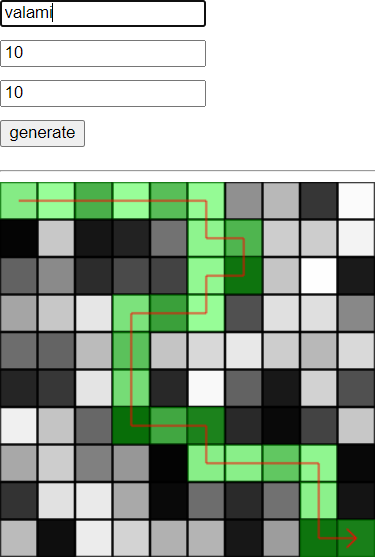
\includegraphics[width=0.34\textwidth]{kepek/map/generate-example-2.png}
				\hspace{5mm}
				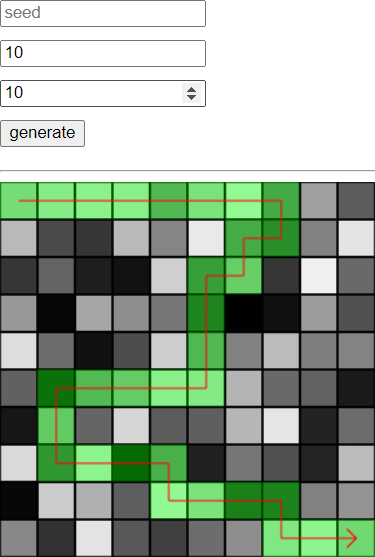
\includegraphics[width=0.34\textwidth]{kepek/map/generate-example-1.png}
				
				\caption{Példák seed-del történő (bal oldal) és anélküli (jobb oldal) pályagenerálásra.}
				\label{fig:map:generateExample}
			\end{figure}
			
			Egy további érdekes része az pályagenerálásnak a cellák forgatásának kezelése. Erre az útvonalnál volt alapvetően szükségem, hiszen a kanyarokat megfelelően beforgatva kellett elhelyezni a pályán. Az alábbi kódrészlet az egyenes útszakaszok megfelelő forgatásának megvalósítását szemlélteti.
			\begin{javascript}
if (§\color{jsConst}d1§ == §\color{jsConst}SIDE\_DOWN§ && §\color{jsConst}d2§ == §\color{jsConst}SIDE\_DOWN§) {
	//straight road, from top to down
	tiles[§\color{jsConst}currentPoint§[0]][§\color{jsConst}currentPoint§[1]] = §\color{jsConst}TILE\_ROAD\_2WAY\_STRAIGHT§ + §\color{jsConst}ROTATION\_ZERO§;
} else if (§\color{jsConst}d1§ == §\color{jsConst}SIDE\_TOP§ && §\color{jsConst}d2§ == §\color{jsConst}SIDE\_TOP§) {
	//straight road, from down to top
	tiles[§\color{jsConst}currentPoint§[0]][§\color{jsConst}currentPoint§[1]] = §\color{jsConst}TILE\_ROAD\_2WAY\_STRAIGHT§ + §\color{jsConst}ROTATION\_ZERO§;
} else if (§\color{jsConst}d1§ == §\color{jsConst}SIDE\_RIGHT§ && §\color{jsConst}d2§ == §\color{jsConst}SIDE\_RIGHT§) {
	//straight road, from left to right
	tiles[§\color{jsConst}currentPoint§[0]][§\color{jsConst}currentPoint§[1]] = §\color{jsConst}TILE\_ROAD\_2WAY\_STRAIGHT§ + §\color{jsConst}ROTATION\_90§;
} else if (§\color{jsConst}d1§ == §\color{jsConst}SIDE\_LEFT§ && §\color{jsConst}d2§ == §\color{jsConst}SIDE\_LEFT§) {
	//straight road, from right to left
	tiles[§\color{jsConst}currentPoint§[0]][§\color{jsConst}currentPoint§[1]] = §\color{jsConst}TILE\_ROAD\_2WAY\_STRAIGHT§ + §\color{jsConst}ROTATION\_90§;
}
			\end{javascript}
			Két esetet különböztettem meg, amikor vízszintesnek kell lennie az útnak, és amikor függőlegesnek. A forgatás értékét a mező értékével együtt tárolom. Ez gyakorlatilag úgy valósul meg, hogy a lebegőpontos szám egész része adja meg a mező képét, a tört része pedig a forgatás értékét. Fontos megemlíteni, hogy a lebegőpontos számábrázolás következtében a törtrész csak a kettő hatványával megadható szám lehet, mert különben veszítünk a pontosságból és nem fog működni a program. Ennek a módszernek az előnye, hogy egy számként kezelve kevesebb memóriát igényel a tárolás és feltehetően gyorsítja a programot is.
		\end{MySubSection}
		
		\begin{MySubSection}{Az effektek}
			Az effektek megvalósítása történt talán a leginkább az OOP elvei szerint, mivel itt nem voltam annyira korlátozva a keretrendszer által, mint máshol. Működésükről annyit érdemes tudni, hogy kezdetben a tornyokon vannak létrehozva, innen továbbkerülnek a lövedékekre, azok pedig az eltalált ellenségekre teszik, ahol végül aktiválódnak is. Miután az ellenfélre kerültek, az adott ellenség minden ciklusban meghívja a rá került effektek update metódusát. Ebben az update metódusban az effekt megfelelő módon módosítja az ellenség tulajdonságait. Ezt úgy valósítottam meg, hogy a meghívott update metódust tovább bontottam egy ``init'', egy ``remove'', és egy másik ``update'' metódusra. Ezek a nevüknek megfelelően a legelső, legutolsó és az összes update ciklusban futnak le. Ezzel lehetőséget nyújtottam többféle effekt készítésére, mint például azonnali hatású, vagy tartós effektekre.
			Implementáció szempontjából fontos volt még, hogy klónozhatóvá tegyük az effekteket, mivel ha nem így lenne, a torony a saját effekt-referenciáját adná tovább az ellenségnek. Ezzel az lenne a probléma, hogy ha több ellenségen lenne ugyanaz az effekt, akkor felülírnák egymás értékeit, illetve az eredeti effektet is felül lehet írni így, ami nem várt eredményeket okozhatna. A klónozás megvalósítása az alábbi kódrészletben látható:
			\begin{javascript}
export abstract class §\color{jsType}BaseCloneable§ implements §\color{jsType}ICloneable§ {
	public abstract §\color{jsMethod}copy§(obj: §\color{jsType}this§): §\color{jsType}this§;
	
	public §\color{jsMethod}clone§(): this {
		const §\color{jsConst}clone§: §\color{jsType}this§ = §\color{jsType}Object§.§\color{jsMethod}create§(§\color{jsType}Object§.§\color{jsMethod}getPrototypeOf§(this));
		§\color{jsConst}clone§.§\color{jsMethod}copy§(this);
		
		return clone;
	}
}
			\end{javascript}
			Az osztály csak a ``clone'' metódust implementálja, melyhez a ``copy'' metódust használja fel, melyet a leszármazottaknak kell majd megadniuk. Látható, hogy mennyire egyszerű is ez a kód a JavaScript környezetben implementálva. Az Object.create() metódus egy adott prototype-nak, vagy osztálynak megfelelő objektumot hoz létre (JavaScriptben az osztályok gyakorlatilag prototype-ok). Ebbe az objektumba pedig belemásoljuk a ``copy'' metódussal az adott példányban található változókat, vagyis a dinamikusan változó részét.
			A következő kódrészletben egy egyszerűbb effektet, a \texttt{FlatDamageEffect}-et láthatjuk. 
			\begin{javascript}
export class §\color{jsType}FlatDamageEffect§ extends §\color{jsType}BaseInstantEffect§ {
	private flatAmount: §\color{jsType}number§;
	
	constructor(flatAmount: §\color{jsType}number§) {
		super();
		this.flatAmount = flatAmount;
	}
	
	protected §\color{jsMethod}init§(enemy: §\color{jsType}IEnemy§): §\color{jsType}void§ {
		super.§\color{jsMethod}init§(enemy, (enemy) => {
			enemy.health -= this.flatAmount;
		})
	}
	
	public §\color{jsMethod}copy§(o: §\color{jsType}this§): §\color{jsType}this§ {
		this.flatAmount = o.flatAmount;
		super.§\color{jsMethod}copy§(o);
		
		return this;
	}
}
			\end{javascript}
			Látható, hogy a ``copy'' metódus az osztályban használt tagokat másolja át az új példányba. Ezután meghívja a szülő ugyanilyen metódusát, hogy az is átmásolhassa a benne definiált tagokat és így tovább, egészen amíg már nincs több szülő. Végeredményben egy teljes értékű másolatot kapunk.
			Az osztály többi része elég könnyedén értelmezhető: az effekt aktiválódása esetén, vagyis az ``init'' metódus lefutása esetén, a konstruktorban megkapott értékkel csökkenti az adott ellenség életerejét. Ha esetleg csak ideiglenesen szeretnénk módosítani az ellenség tulajdonságait, akkor azt a ``remove'' metódussal tudnánk megoldani, ahol vissza kellene állítanunk az eredeti értékeket.

		\end{MySubSection}
		
		\begin{MySubSection}{A GameScene osztály}
			Ez az egyik legfontosabb része a játéknak. Az általános struktúráját követi a Scene osztályoknak, vagyis van ``init'', ``preload'', ``create'' és ``update'' metódusa.
			A Phaser ajánlása szerint az adott képernyőhöz tartozó objektumok megjelenítésének és a hozzá köthető logikának kellene itt szerepelnie, de mivel ez esetünkben nagyon komplex és terjedelmes osztályt eredményezett volna, ezért csak a megjelenítéshez szorosan köthető részeket raktam ide. Tehát itt csak az objektumok létrehozása és a megfelelő paraméterezés kapott helyet. A logikát a \texttt{GameStateStore}-ba helyeztem át. A felhasználói interakciókat az \texttt{Action} osztályok kezelik, a felhasználói felület frissítését pedig callback-ekkel oldottam meg. Az osztály metódusai közül említésre méltó a ``create'', mely az alábbi kódrészletben látható.	
			\begin{javascript}
public §\color{jsMethod}create§(data: {seed: §\color{jsType}string§}): §\color{jsType}void§ {
	const §\color{jsConst}windowSizes§ = this.§\color{jsMethod}getWindowSizes§();
	
	const {§\color{jsConst}map§, §\color{jsConst}path§} = §\color{jsConst}MapGenerator§.§\color{jsMethod}generateMap§(data.seed, §\color{jsConst}MAP\_TILES\_ROW\_COUNT§, §\color{jsConst}MAP\_TILES\_COL\_COUNT§)
	
	const §\color{jsConst}convertedPath§ = this.§\color{jsMethod}getConvertedPath§(§\color{jsConst}path§, §\color{jsConst}windowSizes§);
	this.gameStateStore = new §\color{jsType}GameStateStore§(this, §\color{jsConst}map§, §\color{jsConst}convertedPath§);
	
	this.§\color{jsMethod}createMapTiles§(this.gameStateStore.§\color{jsMethod}getMapDataForTileMap§(), §\color{jsConst}windowSizes§);
	this.§\color{jsMethod}createMapTileSelector§(§\color{jsConst}windowSizes§);
	this.§\color{jsMethod}createMapGrid§(§\color{jsConst}windowSizes§);
	this.§\color{jsMethod}createTopUI§();
	this.§\color{jsMethod}createSideUI§();
	this.§\color{jsMethod}createUIInputHandlers§();
} 
			\end{javascript}
			Mint látható, ebben a metódusban kerül sor a pálya generálására, a ``GameStateStore'' létrehozására, a pálya mezőinek és egyéb részeinek létrehozására és megjelenítésére, valamint a felhasználói felület (UI) létrehozására. Ezek a metódusok nagyrészt csak a Phaser-es objektumokat hozzák létre a megfelelő paraméterekkel. Ami érdekesebb lehet, az a felhasználói felületnél a frissítés és az interakció megoldása. Ezeket mint említettem, callback-ekkel és az \texttt{Action} osztályok segítségével oldottam meg. Lehetett volna más megoldást is alkalmazni, például az ``update'' metódusban folyamatosan lehetett volna frissíteni a felületet és vizsgálni az interakciókat, viszont ez teljesítményben sokkal rosszabb megoldás lett volna. Az alább látható 3 kódrészletben ezeket mutatom be.
			\begin{javascript}
const §\color{jsConst}buttons§ = [
	{
		action: new §\color{jsType}SelectAction§(this.gameStateStore),
		pos: { x: 847.5, y: 145 },
		image: { size: { x: 25, y: 25 }, texture: 'ui', frame: 'select' },
		box: { size: { x: 55, y: 30 }},
	},
	//...
]
			\end{javascript}
			Itt az látható, hogy a felületen megjelenő gombokat majd tömbösítve hozom létre, minden gombhoz megadva pozícióját, képét, méretét és a kattintáskor elvégzendő akciót.
			\begin{javascript}
for (const §\color{jsConst}button§ of §\color{jsConst}buttons§) {
	//...
	§\color{jsConst}interactiveLayer§.§\color{jsMethod}on§(§\color{jsType}Phaser§.§\color{jsType}Input§.§\color{jsType}Events§.§\color{jsConst}POINTER\_OVER§, () => {
		§\color{jsConst}button§.graphics?.boxHover.§\color{jsMethod}setVisible§(true);
	})
	
	§\color{jsConst}interactiveLayer§.§\color{jsMethod}on§(§\color{jsType}Phaser§.§\color{jsType}Input§.§\color{jsType}Events§.§\color{jsConst}POINTER\_OUT§, () => {
		§\color{jsConst}button§.graphics?.boxHover.§\color{jsMethod}setVisible§(false);
	})
	
	§\color{jsConst}interactiveLayer§.§\color{jsMethod}on§(§\color{jsType}Phaser§.§\color{jsType}Input§.§\color{jsType}Events§.§\color{jsConst}POINTER\_DOWN§, () => {
		this.gameStateStore.§\color{jsMethod}setAction§(button.action);
	});
}
			\end{javascript}
			Ez a kódrészlet gombok létrehozásából lett kiragadva. Itt az látható, hogyan reagálok az egéreseményekre, illetve hogy hogyan állítom be a gombnak megfelelő akciót későbbi felhasználásra a \texttt{GameStateStore}-ba (ezek a gombok csak az akció kiválasztásáért felelősek és nem azok futtatásáért).
			\begin{javascript}
this.gameStateStore.actionChangedCallbacks.§\color{jsMethod}push§((action) => {
	§\color{jsConst}buttons§.§\color{jsMethod}forEach§(btn => {
		if(action.actionKey === btn.action.actionKey) {
			btn.graphics?.boxActive.§\color{jsMethod}setVisible§(true);
		} else {
			btn.graphics?.boxActive.§\color{jsMethod}setVisible§(false);
		}
	})
})
			\end{javascript}
			Ebben a kódrészletben pedig az látható, ahogy hozzáadok a \texttt{GameStateStore}-hoz egy callback-et, ami akkor fog lefutni ha megváltozik a kiválasztott akció. Erre azért van szükség mert mindig az éppen aktuális akciónak megfelelő gombot jelenítjük meg másképp (kijelölve). Ezt a callback-es módszert egyébként is előszeretettel alkalmazzák más JavaScript alapú alkalmazásoknál, illetve weboldalak készítésénél is.
		\end{MySubSection}
		
		\begin{MySubSection}{A finomhangolás}
			A fejlesztés legutolsó szakasza volt ez, mely során az elkészült játék paramétereit módosítgattam a megfelelő nehézségi egyensúly eltalálásához. Ezt gyakorlatilag próba-szerencse módon végeztem több-kevesebb sikerrel. A változtatott értékek többek között a tornyok sebzése, tűzgyorsasága, ára, az ellenségek ereje, pénzértéke, stb. volt. Mivel ez egy sokváltozós feladat és nehezen megfogható objektívan mi számít kellően nehéznek, de még élvezetesnek egyesek számára, így nem is törekedtem a tökéletességre.
			A kezdetben jónak tűnő értékek nagyon könnyű játékot eredményeztek, konkrétan 1-2 rakétavetős torony lerakásával végtelenségig játszható lett volna a játék, szóval ezen mindenképp javítani kellett. A végeredményben számomra még mindig könnyűnek tűnő játékot kaptam, de az előzőekhez képest már érezhető volt a javulás.
		\end{MySubSection}
			
	\end{MySection}
	
	\begin{MySection}{Tesztelés}
		A tesztelés egy fontos folyamat, mind alkalmazások készítésénél, mind pedig játékfejlesztés esetében. 
		A szakdolgozatom részeként készített játékban elsődlegesen a Jest NPM package segítségével próbáltam megvalósítani a tesztelés nagy részét, azonban ez elég nehézkes volt, mert a Phaser és a Jest nem teljesen kompatibilis egymással.
		
		A Jest működéséhez fontos megemlíteni a \textit{jest.mock(...)}, \textit{jest.fn()}, \textit{mock.clear()}, \textit{mock.reset()} és \textit{expect(...)} metódusokat.
		A \textit{jest.mock(path, impl)} a paraméterként megadott modult fogja mockolni vagy automatikusan, vagy az opcionálisan megadott implementáció szerint.
		A \textit{jest.fn()} egy mock (ál) metódust hoz létre, mellyel lehet befolyásolni a metódus működését, illetve ellenőrizni a használatát.
		A \textit{mock.clear()} a mockban tárolt adatokat törli ki, mint például a függvény hívások száma és a beadott paraméterek értéke.
		A \textit{mock.reset()} az előzőhöz hasonlóan működik, annyi plusszal, hogy a mock implementációját is visszaállítja az eredetileg megadottra.
		Az \textit{expect(...)}-el lehet különböző értékeket vizsgálni, az egyszerű változó egyenlőségtől, egészen a mock függvények meghívásainak ellenőrzéséig rengeteg mindent.
		
		A keretrendszer miatt alapjában véve szinte lehetetlen volt mindent lefedni a tesztekkel, mert bizonyos dolgok tesztelését határozottan megnehezíti.
		Gondolok itt például arra, hogy a Phasert lényegében nem lehet automatikusan mockolni, mert ilyen esetben hibára fut a Jest, tehát ekkor csak manuálisan van erre lehetőségünk, a keretrendszer minden szükséges részét megfelelően implementálva.
		
		További problémát jelentett még, hogy a Phaser alapvetően csak egyetlen helyen volt beimportálva, konkrétan a main osztályban, így a Jest csak ott tudta volna kicserélni az implementációját, ez viszont lehetetlenné tette volna a többi osztálynak a main-től független tesztelését. Ez, hogy csak egy helyen legyen beimportálva a Phaser, a weboldalukon \cite{phaser_official_website} található tutoriálokban, példakódokban, dokumentumokban, valamint a \url{https://blog.ourcade.co/} blogon lévő leírásokban kifejezetten fel volt tüntetve, mert problémákat okozhat, ha véletlenül kétszer is importálásra kerül a framework. Ezt megoldandó, készítettem egy úgynevezett wrapper osztályt, ami pontosan egyszer importálja be a Phaser-t, amit így akár több helyen is biztonsággal lehet használni a Phaser használatára.
		
		Egy feltehető bug-ot (hibát) is találtam a Jest-ben: azoknál a metódusoknál melyek az input paramétereiket módosítják, nem lehet helyesen ellenőrizni mivel lettek meghívva, mert a Jest nem tárolja el az eredeti értékét a paramétereknek. Ez esetemben kiküszöbölhető volt a metódus módosításával, de ez nem minden esetben lenne megtehető.
			
		Nehézség volt még, hogy az ES6-os (ECMAScript 6) osztályok mockolása kicsit problémás a Jest-tel, ezért készítettem egy \texttt{MockHelper} nevezetű osztályt, ami ezt orvosolja. A probléma abból fakadt, hogy a \texttt{jest.mock(...)} metódusba jelen állás szerint nem lehet külső változókat használni, tehát itt előre meg kell adni az osztály implementációját, viszont valamiért utólag (a konkrét teszt során) már nem lehet módosítani ezt az implementációt. Ezt úgy tudtam megkerülni, hogy közvetlenül az osztály prototype-ját módosítom ideiglenesen, és ennek az egyszerű és biztonságos kezelésére készült el az említett helper osztály.	

		% hogyan teszteltél leírni
			% - manuális teszelés: vagyis hogy kipróbáltam kézzel hogy jól működnek a funkciók, ez volt nagyrészt a fejlesztés folyamán
		A lefedés tekintetében inkább a lényegesebb, több gondolkodást igénylő részek lefedése volt a célom. A fejlesztés során nagyrészt manuálisan teszteltem, azaz kipróbáltam kézzel, hogy jól működnek-e a funkciók. Tehát elsődlegesen csak akkor írtam tesztet, ha a bonyolultság miatt szükségesnek érződött, a tesztek nagy része azonban csak a játék elkészülte után íródott, akkor integráltam a kész kódhoz.
		Az előbb említett bonyolultabb részek alatt értem például a pályagenerálást, pontosabban azt, hogy az helyesen működik-e, melyről alább látható egy kódrészlet.
		\begin{javascript}
§\color{jsMethod}test§('Test seed same generated map', () => { //...
§\color{jsMethod}test§('Test seed different generated map', () => { //...
§\color{jsMethod}test§('Test proper dimensions', () => { //...
§\color{jsMethod}test§('Test proper map values', () => { //...
§\color{jsMethod}test§('Test proper path start & end', () => { //...
§\color{jsMethod}test§('Test proper path values', () => { //...
§\color{jsMethod}test§('Test path no crossings', () => { //...
§\color{jsMethod}test§('Test path connected', () => { //...				
		\end{javascript}
		A kódrészletbe a tesztesetek neveit tettem bele szemléltetésképpen, hogy látható legyen milyen dolgokat vizsgáltam a pályagenerálás esetében.
		Ez, mint ahogy a \myref{fig:test:mapgen} képen is látható, hasznos volt, hiszen fény derült egy hibára az útvonal mezőinek forgatásával kapcsolatban.
			
 		\begin{figure}[H]
	 		\centering
	 		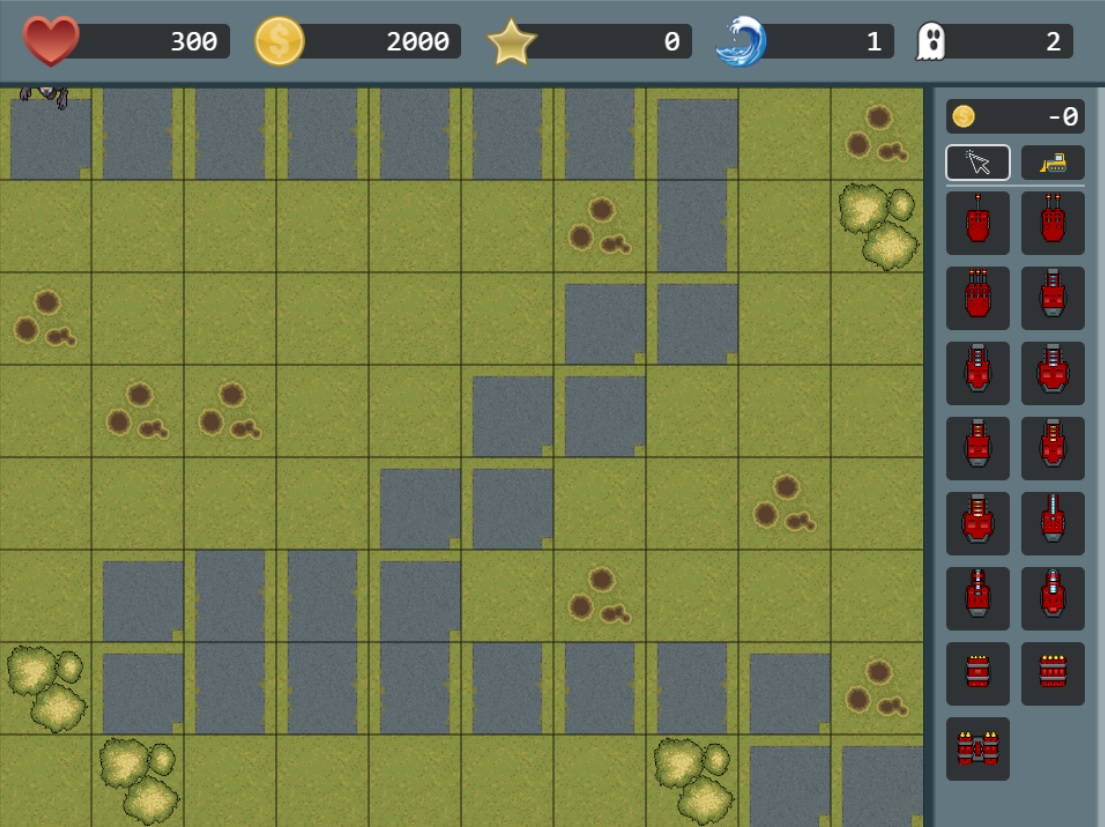
\includegraphics[scale=0.5]{kepek/teszt/tesztRosszPelda}
		 	\caption{A rosszul működő pályagenerálás}
		 	\label{fig:test:mapgen}
		\end{figure}
	
		A felhasználói felület (User Interface röviden: UI), illetve a megjelenítés könnyen módosítható kell, hogy legyen a jövőben is, ezért nem feltétlenül lett volna értelme részletesen, akár pixelre pontosan letesztelni. 
		Ebből kifolyólag a teljesség igénye nélkül, ahol érdemesebbnek tartottam, ott nagyvonalakban néhány dolgot lefedtem, ezáltal tehát nem teljesen tökéletes a teszt lefedettség, de nem is feltétlenül ez volt a cél.
		
		Végül viszonylag sok tesztet sikerült írnom, összesen $189$-et, melyekről egy futtatás a \myref{fig:test:run} képen látható. Innen az is leolvasható, hogy sokáig, majdnem egy teljes percig futottak a tesztek. Ennek feltételezhető oka nem a program komplexitása, hanem inkább a Phaser és a Jest inkompatibilitása.
		
 		\begin{figure}[H]
			\centering
			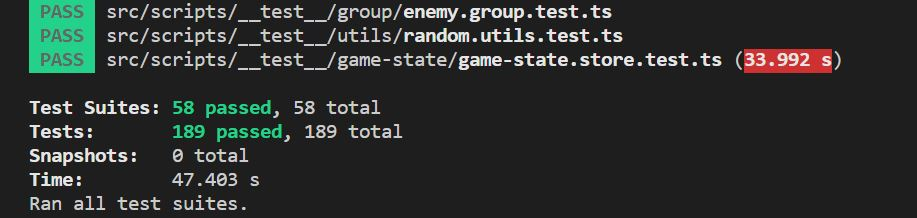
\includegraphics[scale=0.75]{kepek/teszt/testFuttatas}
			\caption{A tesztek futtatása}
			\label{fig:test:run}
		\end{figure}
	
		Az összességében elért teszt lefedettség a \myref{tab:teszt_lefedettseg} táblázatban látható. Az objektumok nagyrészt nem lettek letesztelve, mert sajnos már nem jutott rá idő, így ez rontja az összességében elért eredményt, ezt az ``All files'' sorban találjuk. Éppen ezért a táblázatba belefoglaltam az objektumok tesztelési lefedettsége nélküli végeredményeket is, melyek pedig a ``Without objects module'' sorban láthatóak, így lényegesen nagy különbség figyelhető meg az értékek között.
		A ``Lines'' oszlop azt tartalmazza, hogy a programban szereplő soroknak hány százaléka lett letesztelve, a ``Functions'' a játékban használatos függvények tesztelésének lefedettségét jelzi.
		A ``Statemens'' oszlopban a program logikailag legkisebb futtatható egységeinek teszteltségét láthatjuk.
			% pl fgv hívás amiben van 1 változó ami meg van szorozva 2-vel pl, több sorban lehet tagolva de egy futtatható egység, itt a szorzás pedig egy kifejezés(expression)
		A ``Branches'' alatt pedig az elágazások ágainak lefedettségét értjük.
			
		\begin{table}[h]
			\centering
			\caption{Teszt lefedettség az összes fájllal, majd az objektumokat nem számítva.}
			\label{tab:teszt_lefedettseg}
			\begin{tabular}{l|c|c|c|c|}
				\cline{2-5}
				& Statements & Branches & Functions & Lines \\ \hline
				\multicolumn{1}{|l|}{All files} & 66.67\% & 48.8\% & 52.22\% & 66.89\% \\ \hline
				\multicolumn{1}{|l|}{Without objects module} & 85.89\% & 73.4\% & 72.22\% & 86.2\% \\ \hline
			\end{tabular}
			% https://www.tablesgenerator.com/
		\end{table}
		
	\end{MySection}

	\begin{MySection}{Használat}
		% játék/program bemutatása
		% Felhasználói kézikönyv jellegű leírás. Kifejezetten a végfelhasználó szempontjából lehet azt bemutatni, hogy mit hogy lehet majd használni.
		A továbbiakban az elkészült játékot fogom bemutatni, részletesen leírom a használatát a végfelhasználó szempontjából, képekkel mellékelve.
		
		A játék elindításakor, miután minden betöltődött, a főmenübe kerülünk. (A töltés haladását a töltő képernyőn nyomon követhetjük.)

		A menüben egy ``Generate map'' feliratot láthatunk elsőként, alatta egy szövegdobozzal, melyben a következő szöveg található: ``seed''. Ezek pontos kinézetét a \myref{fig:jatekHasznalat:fomenu} ábrán láthatjuk. Felhasználóként itt van lehetőségünk beírni akármilyen karaktert, szöveget de akár üresen is hagyhatjuk. Ezzel a bemeneti értékkel tudjuk változtatni a generált pályát, amelyen majd játszani fogunk.
		Ennek jobb oldalán egy gomb helyezkedik el, rajta dobókocka ábrákkal. Amennyiben nem szeretnénk gondolkodni, hogy mit írjunk be a szövegdobozba, erre kattintva az alkalmazás véletlenszerűen generálni fog nekünk egy úgynevezett seed-et.
		A seed a pályák egyediségéért felel, amennyiben ugyanazt a seed-et használjuk többször, azonos pályát fog generálni az alkalmazás, így ugyanazon a pályán játszhatunk újra meg újra. Ha viszont különböző bemenetet adunk meg seed-ként, akkor mindig más pályát kapunk végeredményként. 
		Amennyiben beírtuk, vagy legeneráltuk a használni kívánt seed-et, a ``Play'' gombra kattintva tudjuk elindítani a játékot.
		
		\begin{figure}[H]
			\centering
			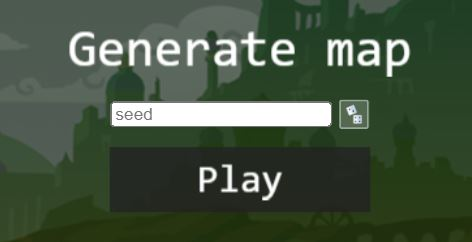
\includegraphics[scale=0.63]{kepek/jatekHasznalat/fomenu}
			\caption{Illusztráció a játék főmenüjéből}
			\label{fig:jatekHasznalat:fomenu}
		\end{figure}
		
		A játék megkezdése után egy másik képernyőn találjuk magunkat, amelyen különféle elemeket láthatunk. Egy példát erre a \myref{fig:jatekHasznalat:game_scene} ábrán tekinthetünk meg. Itt különböző tájelemek helyezkednek el, kráterek, fák, és sima fűvel borított területek, ezenkívül pedig egy útvonal. 
		
		\begin{figure}[H]
			\centering
			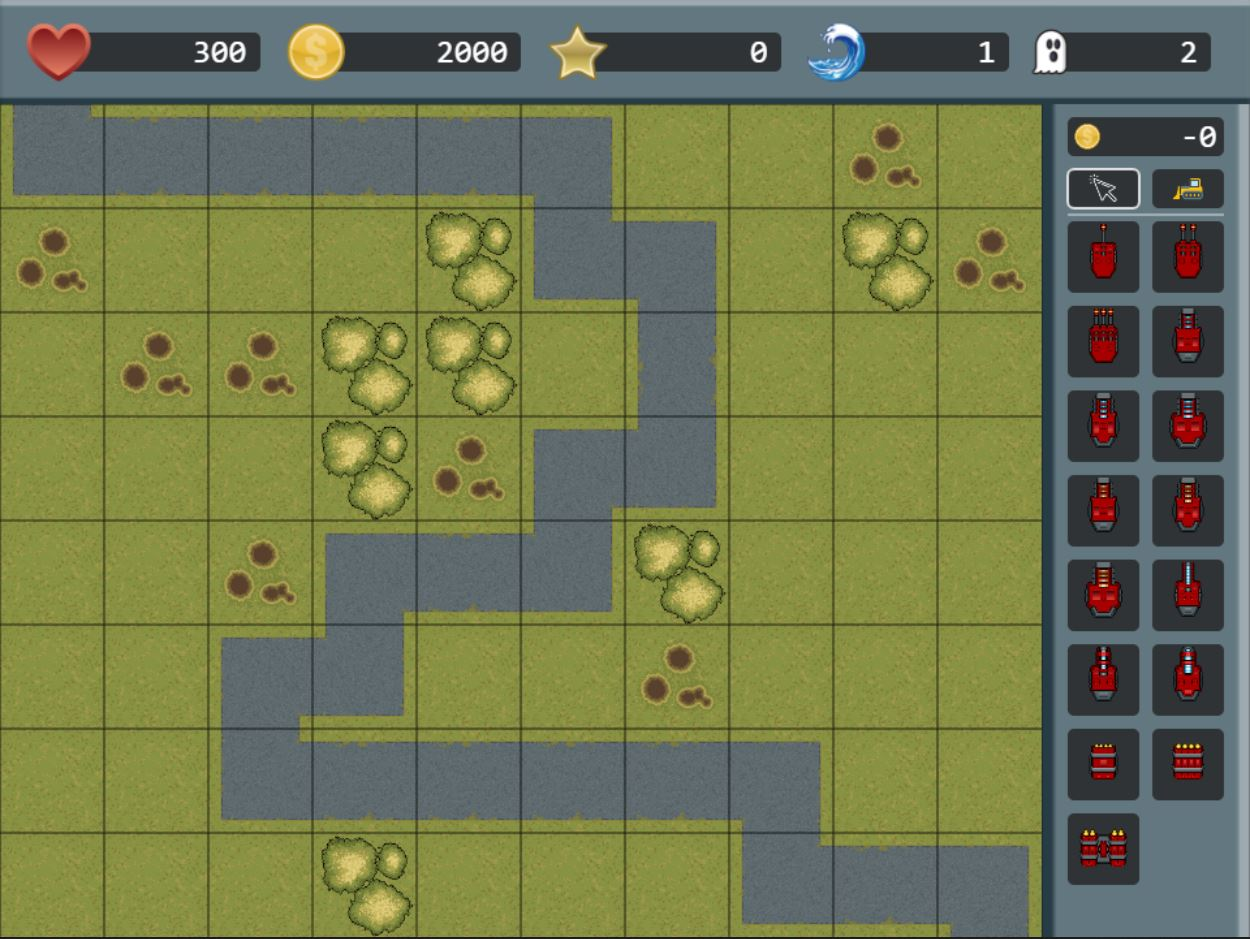
\includegraphics[scale=0.45]{kepek/jatekHasznalat/game_scene}
			\caption{A játék közvetlenül elindítás után}
			\label{fig:jatekHasznalat:game_scene}
		\end{figure}
		
		Az úton szörnyek (lásd: \myref{fig:jatekHasznalat:szorny} ábra) fognak elindulni, pár másodperccel a játék elindítása után, és megpróbálnak végigmenni rajta.
		A feladatunk az, hogy megakadályozzuk őket ebben. Ezt úgy tudjuk megtenni, hogy különféle tornyokat helyezünk le, ezek fogják sebezni a szörnyeket.
		Az ellenségek feje fölött egy-egy zöld csík látható, amikor megjelennek, ez az életüket szimbolizálja. Amennyiben sebzést szenvednek el, a zöld rész egyre kisebb lesz, amikor pedig teljesen elfogy, a szörny meghal. Az ellenfelek hullámokban, avagy hordaként érkeznek. Minden hullámmal egyre több, és erősebb ellenség fog érkezni.
		
		\begin{figure}[H]
			\centering
			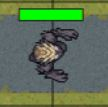
\includegraphics[width=0.12\textwidth]{kepek/jatekHasznalat/szorny}
			\caption{Az ellenfél}
			\label{fig:jatekHasznalat:szorny}
		\end{figure}
		
		Tornyokat csak üres, füves területekre tudunk építeni. Amennyiben nincs már hely ahova tudnánk tenni, le is rombolhatunk előzőleg épülteket, vagy pedig a tájelemeket is. Ezt a jobb oldalt látható felület által tehetjük meg (lásd: \myref{fig:jatekHasznalat:game_scene} ábra jobb oldala).		
		A játék kezdetekor az egér ikont ábrázoló gomb van kijelölve. Ez az úgynevezett ``kijelölés mód'' gomb, ha ezen a módon belül vagyunk, tehát ez a gomb van bekeretezve fehér színnel, akkor ha egy már megépült toronyra rávisszük a kurzort, látni fogjuk a hatótáv jelölő kört körülötte. Ezen a körön belüli távolságra lévő ellenfeleket képes elérni a torony. % A "kijelölés mód"-ban az egyes objektumokra kattintva a játékon belül nem történik semmi, szimplán amelyik mező felett van a kurzorunk, az lesz kijelölve.
		Az ettől jobbra található, sárga buldózer ábrával ellátott gombra kattintva pedig az ``eltávolító mód''-ba kerülünk. Ha ebben a módban vagyunk, és odamozgatjuk a kurzort (kattintás nélkül) egy-egy tárgyra a játékfelületen belül, akkor amíg az adott tárgy fölött van az egerünk, addig az előbb említett gombok feletti rubrikában látható, hogy amennyiben le szeretnénk rombolni az adott objektumot, milyen összeggel változna a pénzünk, avagy aranyunk. Az objektum tényleges eltávolítása kattintásra történik meg.
		Abban az esetben, ha egy korábban megépített tornyot szeretnénk megsemmisíteni, a torony eredeti értékének 60\%-át kapjuk vissza, tehát például ha egy toronyért 1000 aranyat fizettünk, amikor rávisszük a kurzort eltávolító módban, $+600$-at fogunk látni a rubrikában, tehát 600 aranyat kapunk vissza, a rombolás után. Ellenben kráter, vagy fa eltávolításához fizetnünk kell a rombolásért, tehát egy mínuszjel után fog megjelenni az összeg, amennyibe kerül.
		A két gomb alatti felületen különféle tornyok helyezkednek el, 5 különböző típusú tornyot tudunk építeni, és mind az 5 típusból létezik 3 különböző erősségű.
		A tornyok balról jobbra vannak sorba rendezve, tehát adott típusú toronynak először a leggyengébb változatát láthatjuk, a végén pedig a legerősebbet, de összességében szituációfüggő is, hogy épp melyik az, amit a legjobban megéri építenünk. Az azonos típusú tornyok hasonló megjelenéssel rendelkeznek, hogy látható legyen az, hogy egy ugyanazon típuson belül helyezkednek el, az áruk azonban különböző.
		
		Az egyes tornyok tulajdonságairól részletesebb leírás alább, a fejezet végén lévő táblázatokban olvasható (lásd: \myref{tab:torony_tipus_0}, \myref{tab:torony_tipus_1}, \myref{tab:torony_tipus_2}, \myref{tab:torony_tipus_3}, \myref{tab:torony_tipus_4} táblázatok).
		
		% mindegyik torony - táblázat, a torony képével, képességeivel, árával stb.
		% Tűzgyorsaság helyett-> lövés/sec -> 2 lövés között 1000/firerate-nyit vár 
	
		A felső felhasználói felületen (lásd \myref{fig:jatekHasznalat:felso_ui} ábra) balról jobbra haladva, a következőket láthatjuk:
		
		\begin{figure}[H]
			\centering
			
\includegraphics[scale=0.58]{kepek/jatekHasznalat/felso_ui}
			\caption{A felülső felhasználói felület (UI) }
			\label{fig:jatekHasznalat:felso_ui}
		\end{figure}
		
		\begin{itemize}
			\item Piros szív ábra: Az itt látható szám az aktuális életerőnket jelzi. Ez csökkenni fog, ha egy szörnyet engedünk végigmenni az egész úton. Amikor teljesen elfogy, akkor veszítünk, az adott játék véget ér.
			
			\item Sárga érme ``\$'' jellel: Ebben a rubrikában az aktuális aranyunk jelenik meg. Ez az érték többször is változhat a játék során. Például toronyépítéskor levonódik a torony összege, ellenben amikor megölünk egy szörnyet akkor kapunk érte adott aranymennyiséget.
			
			\item Csillag ikon: A pillanatnyi összpontszámunkat mutatja. Minden ellenfél megölése után kapunk adott mennyiségű pontot. A végeredményként elért összpontszámot a játék vége után is megtekinthetjük, mielőtt visszalépünk a főmenübe.
			
			\item Hullám: Azt jelzi, hogy hányadik beérkező hordánál, szörnyhullámnál tartunk éppen.
			
			\item Szellem ikon: A szörnyeket jelképezi. Azt jelzi a játékos számra, hogy az adott hullámban mennyi ellenség érkezik.
		\end{itemize}
	
		A fentieken kívül még megemlítendő, hogy amennyiben olyan tevékenységet kívánunk tenni, amely nem lehetséges az adott mezőben, (például nincs elég pénzünk, hogy megvegyük a jobb oldali menüből kiválasztott tornyot, vagy mondjuk ha az utat próbáljuk meg eltávolítani), úgy a mező pirosas színre vált, ha pedig lehetséges az akció végrehajtása, akkor élénk zöldes árnyalatot kap. A (\myref{fig:jatekHasznalat:kijeloles_minta} ábrán bal oldalt az előbbi, jobb oldalt pedig az utóbbi látható.)
		
		\begin{figure}[H]
			\centering
			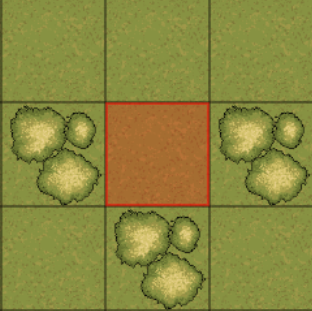
\includegraphics[scale=0.858]{kepek/jatekHasznalat/minta_rossz_kijeloles}
			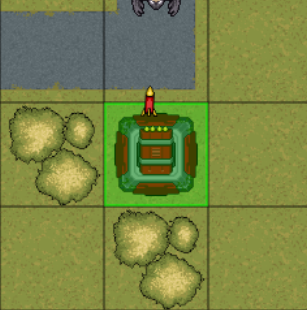
\includegraphics[scale=0.86]{kepek/jatekHasznalat/minta_jo_kijeloles}
			\caption{Minta kijelölésekre - lehetetlen, illetve teljesíthető akciók esetén}
			\label{fig:jatekHasznalat:kijeloles_minta}
		\end{figure}
		
		% game over scene
		
		Most, hogy elolvastuk az előbbieket, már mindent tudunk a játékmenetről. Ami tehát még hátravan, az az, hogy mi történik akkor, amikor esetlegesen elveszítjük az összes életünket, ezáltal a játékot is.
		Ekkor egy új felület jelenik meg előttünk (lásd: \myref{fig:jatekHasznalat:game_over_scene} ábra), amelyen egy ``Game Over'' felirat található, emellett itt megtekinthetjük a játék során elért összpontszámunkat, valamint a ``Back to Main Menu'' gombra kattintva pedig újra a főmenübe navigálhatjuk magunkat, hogy belekezdhessünk egy új játékmenetbe.
		
		\begin{figure}[H]
			\centering
			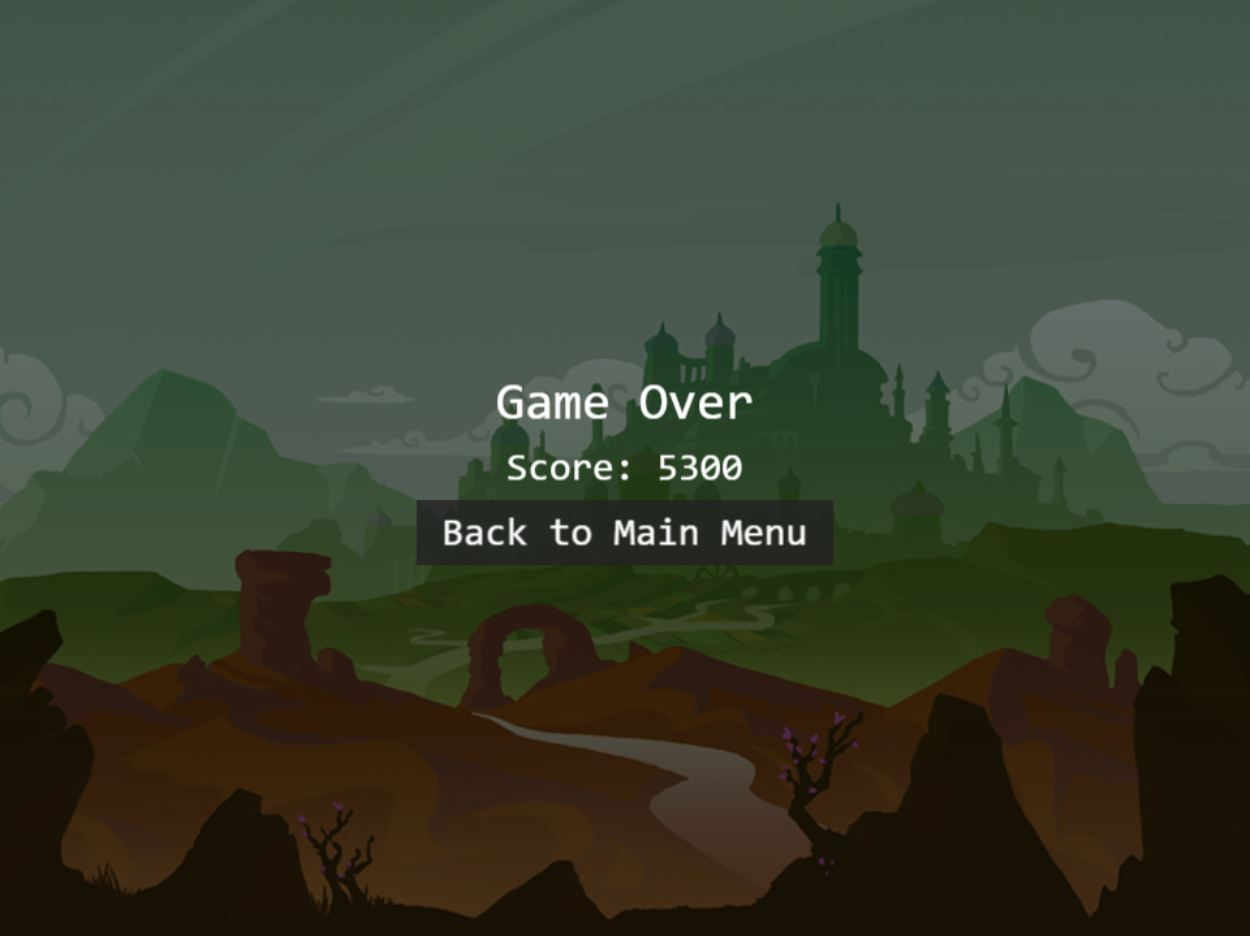
\includegraphics[scale=0.5]{kepek/jatekHasznalat/game_over_scene}
			\caption{Részlet a Game Over képernyőről}
			\label{fig:jatekHasznalat:game_over_scene}
		\end{figure}

		\begin{table}[H]
			\centering
			\caption{Első toronytípus tulajdonságai}
			\label{tab:torony_tipus_0}
			\begin{tabular}{|l|C{2.9cm}|C{2.9cm}|C{2.9cm}|}
				\hline
				Kinézet & 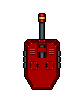
\includegraphics[scale=0.76]{kepek/jatekHasznalat/torony_01} & 
\includegraphics[scale=0.76]{kepek/jatekHasznalat/torony_02} & 
\includegraphics[scale=0.76]{kepek/jatekHasznalat/torony_03} \\ \hline
				Ár (arany) & 500 & 1200 & 3000 \\ \hline
				Maximum lőtávolság & 220 & 250 & 280 \\ \hline
				Lövés/sec & 2 & 1.6 & 1.4 \\ \hline
				Sebzés & 25 & 25 & 25 \\ \hline
				% Százalékos sebzés & Nincs & Nincs & Nincs \\ \hline
				Képesség, effekt & Egy lövésnél 1 lövedéket lő ki. & Egy lövésnél 2 lövedéket lő ki. & Egy lövésnél 3 lövedéket lő ki. \\ \hline
			\end{tabular}
		\end{table}
		
		\begin{table}[H]
			\centering
			\caption{Második toronytípus tulajdonságai}
			\label{tab:torony_tipus_1}
			\begin{tabular}{|l|C{2.85cm}|C{3.06cm}|C{3.06cm}|}
				\hline
				Kinézet & 
\includegraphics[scale=0.78]{kepek/jatekHasznalat/torony_11} & 
\includegraphics[scale=0.78]{kepek/jatekHasznalat/torony_12} & 
\includegraphics[scale=0.78]{kepek/jatekHasznalat/torony_13} \\ \hline
				Ár (arany) & 800 & 1600 & 3200 \\ \hline
				Maximum lőtávolság & 220 & 250 & 280 \\ \hline
				Lövés/sec & 1.4 & 1.4 & 1.4 \\ \hline
				Sebzés & 10 & 10 & 10 \\ \hline
				% Százalékos sebzés & Nincs & Nincs & Nincs \\ \hline
				Képesség, effekt & Lassító lövedéket lő ki. & 1-es átütő- képességű lassító lövedéket lő ki. & 2-es átütő- képességű lassító lövedéket lő ki. \\ \hline
			\end{tabular}
		\end{table}
	
		\begin{table}[H]
			\centering
			\caption{Harmadik toronytípus tulajdonságai}
			\label{tab:torony_tipus_2}
			\begin{tabular}{|L{3.75cm}|C{3.07cm}|C{3.06cm}|C{3.06cm}|}
				\hline
				Kinézet & 
\includegraphics[scale=0.63]{kepek/jatekHasznalat/torony_21} & 
\includegraphics[scale=0.63]{kepek/jatekHasznalat/torony_22} & 
\includegraphics[scale=0.63]{kepek/jatekHasznalat/torony_23} \\ \hline
				Ár (arany) & 800 & 1600 & 3200 \\ \hline
				Maximum lőtávolság & 220 & 250 & 280 \\ \hline
				Lövés/sec & 1.4 & 1.4 & 1.4 \\ \hline
				Sebzés & 10 & 10 & 10 \\ \hline
				% Százalékos sebzés & Nincs & Nincs & Nincs \\ \hline
				Képesség, effekt & Tüzes lövedéket lő ki.(DOT-ként) & 1-es átütő- képességű tüzes lövedéket lő ki. & 2-es átütő- képességű tüzes lövedéket lő ki. \\ \hline
			\end{tabular}
		\end{table}
	
		%\begin{remark}
		%	Ez egy megjegyzés
		%\end{remark}
		%\footnotetext{DOT: Damage Over Time, magyarul olyan sebzésforma, amely nem egyszer sebez, hanem bizonyos időn keresztül folyamatosan sebzi az ellenfelet.}
	
		\begin{table}[H]
			\centering
			\caption{Negyedik toronytípus tulajdonságai}
			\label{tab:torony_tipus_3}
			\begin{tabular}{|L{3.75cm}|C{2.9cm}|C{2.9cm}|C{2.9cm}|}
				\hline
				Kinézet & 
\includegraphics[scale=0.63]{kepek/jatekHasznalat/torony_31} & 
\includegraphics[scale=0.63]{kepek/jatekHasznalat/torony_32} & 
\includegraphics[scale=0.63]{kepek/jatekHasznalat/torony_33} \\ \hline
				Ár (arany) & 700 & 1400 & 2800 \\ \hline
				Maximum lőtávolság & 220 & 250 & 280 \\ \hline
				Lövés/sec & 1.4 & 1.6 & 2.0 \\ \hline
				% Sebzés & 0 & 0 & 0 \\ \hline
				Százalékos sebzés & 20 \% & 20 \% & 20 \% \\ \hline
				Képesség, effekt & \multicolumn{3}{c|}{Instant sebez, egyszerre egy ellenséget, lézersugárral.} \\ \hline
			\end{tabular}
		\end{table}
	
		\begin{table}[H]
			\centering
			\caption{Ötödik toronytípus tulajdonságai}
			\label{tab:torony_tipus_4}
			\begin{tabular}{{|L{3.88cm}|C{2.7cm}|C{2.7cm}|C{2.7cm}|}}
				\hline
				Kinézet & 
\includegraphics[scale=0.65]{kepek/jatekHasznalat/torony_41} & 
\includegraphics[scale=0.65]{kepek/jatekHasznalat/torony_42} & 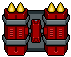
\includegraphics[scale=0.65]{kepek/jatekHasznalat/torony_43} \\ \hline
				Ár (arany) & 1000 & 2500 & 4000 \\ \hline
				Maximum lőtávolság & 220 & 250 & 280 \\ \hline
				Lövés/sec & 1.0 & 1.05 & 1.1 \\ \hline
				Sebzés & 10 & 10 & 10 \\ \hline
				Százalékos sebzés & 10 \% & 10 \% & 10 \% \\ \hline
				Képesség, effekt & \multicolumn{3}{C{8.8cm}|}{Rakétát lő ki, becsapódáskor a robbanás hatósugarában tartózkodó összes ellenfelet sebzi.} \\ \hline
				Robbanás hatósugara & 50 & 75 & 100 \\ \hline
			\end{tabular}
		\end{table}
	
	\end{MySection}

\end{MyChapter}